\chapter{最优体积约束比}
TODO
针对体积约束比和LBB稳定性条件验证方法的局限性,本章采用泛函分析的手段,验证LBB稳定性条件与特征值问题的等价性。
详细讨论特征值问题非零特征值个数与体积约束比之间的联系,从而建立体积约束比和LBB稳定性条件之间的关系。
以此,构建考虑体积约束比的新型LBB稳定系数估计表达式,从而确定最优体积约束比。

\section{LBB稳定性条件与特征值问题}

基于LBB稳定性条件\eqref{infsup},假设$\mathcal P_h:V_h \rightarrow Q_h$ 是$\mathcal P$的正交投影算子,定义为:
\begin{equation}\label{Ph}
    b(q_h,\boldsymbol v_h) = (q_h, \mathcal P \boldsymbol v_h) = (q_h, \mathcal P_h \boldsymbol v_h), \quad \forall q_h \in Q_h
\end{equation}
式中, 散度算子$\mathcal P:V\rightarrow Q$ , $\mathcal P = \nabla \cdot$。

根据$\mathcal P_h$的定义,有$\mathrm{Im}\mathcal P_h \in Q_h$。式\eqref{infsup}可以改写为:
\begin{equation} \label{r11}
    \begin{split}
        \beta &\le \inf_{q_h \in Q_h} \sup_{\boldsymbol v_h \in V_h} \frac{\vert b(q_h,\boldsymbol v_h) \vert}{\Vert q_h \Vert_Q \Vert \boldsymbol v_h \Vert_V} 
        \le \inf_{q_h \in \mathrm{Im}\mathcal P_h} \sup_{\boldsymbol v_h \in V_h} \frac{\vert (q_h,\mathcal P_h \boldsymbol v_h) \vert}{\Vert q_h \Vert_Q \Vert \boldsymbol v_h \Vert_V} \\
    \end{split}
\end{equation}

对于给定的 $q_h\in \mathrm{Im}\mathcal P_h$,假设空间$V'_h \subset V_h\setminus \ker P_h$定义为:
\begin{equation}
    V'_h = \{ \boldsymbol v_h \in V_h \; \vert \; \mathcal P_h \boldsymbol v_h = q_h \}
\end{equation}
由 $\mathrm{Im}\mathcal P_h \in Q_h$,根据柯西--施瓦茨不等式,有
\begin{equation}
    \vert (q_h,\mathcal P_h \boldsymbol v_h) \vert \le \Vert q_h \Vert_Q \Vert \mathcal P_h \boldsymbol v_h \Vert_Q
\end{equation}
同时,当且仅当$q_h=\mathcal P_h \boldsymbol v_h$时,等式成立,即
\begin{equation}
    \vert (q_h,\mathcal P_h \boldsymbol v_h) \vert = \Vert q_h \Vert_Q \Vert \mathcal P_h \boldsymbol v_h \Vert_Q, \quad \forall \boldsymbol v_h \in V'_h
\end{equation}
代入到式\eqref{r11}中可得:
\begin{equation}\label{r12}
    \sup_{\boldsymbol v_h\in V_h} \frac{\vert (q_h,\mathcal P_h \boldsymbol v_h) \vert}{\Vert q_h \Vert_Q \Vert \boldsymbol v_h \Vert_V} =
    \sup_{\boldsymbol v_h\in V'_h} \frac{\Vert \mathcal P_h \boldsymbol v_h \Vert_Q}{\Vert \boldsymbol v_h \Vert_V} 
\end{equation}

结合式\eqref{r11}、\eqref{r12}可得LBB稳定系数估算式:
\begin{equation}\label{r1}
    \beta \le \inf_{V'_h \subset V_h \setminus \ker \mathcal P_h} \sup_{v_h \in V'_h} \frac{\Vert \mathcal P_h \boldsymbol v_h \Vert_Q}{\Vert \boldsymbol v_h \Vert_V}
\end{equation}
其中 $\ker \mathcal P_h \subset V$ 是 $\mathcal P_h$ 的核,定义为 $\ker \mathcal P_h := \{ \boldsymbol v \in V \;\vert\; \mathcal P_h \boldsymbol v = 0 \}$.

上述方法与传统数值inf--sup测试一致\cite{malkus1981},而根据极小--极大值原理 \cite{babuska1991a},式\eqref{r1}计算刚度矩阵$\boldsymbol K^v$ 和 $\boldsymbol K^d$的最小非零特征值。
\subsection{特征值问题与体积约束比}

为了进一步找出最优约束自由度数量,引入完备多项式空间$P_{n_u}$ 是一个$n_u$ 维的多项式空间, $V_{n_u}$ 是位移多项式空间,且 $V_{n_u} = P_{n_u}^2$。由于$V_h$ 和 $V_{n_u}$的维度相同,$\dim V_{n_u}=\dim V_h = n_d\times n_u$,存在一个唯一的$\boldsymbol v \in V_{n_u}$ 满足$\boldsymbol v_h = \mathcal I_h \boldsymbol v$。于是式\eqref{r1}的右边可以改写为:
\begin{equation}\label{r21}
    \inf_{V'_h \subset V_h\setminus \ker \mathcal P_h}\sup_{\boldsymbol v_h \in V_h'} \frac{\Vert \mathcal P_h \boldsymbol v_h \Vert_Q}{\Vert \boldsymbol v_h \Vert_V} = 
    \inf_{V'\subset V_{n_u}\setminus \ker \mathcal P_h \mathcal I_h}\sup_{\boldsymbol v \in V'} \frac{\Vert \mathcal P_h \mathcal I_h \boldsymbol v \Vert_Q}{\Vert \mathcal I_h \boldsymbol v \Vert_V}
\end{equation}
压力的自由度为$n_p = \dim(V_{n_u}\setminus \ker \mathcal P_h \mathcal I_h)$

根据三角不等式、柯西--施瓦茨不等式和式\eqref{Ph}中的等式关系可得:
\begin{equation}\label{interpolation1}
    \begin{split}
        \Vert \mathcal P_h \mathcal I_h \boldsymbol v \Vert_Q &= 
        \sup_{q_h \in Q_h} \frac{\vert (q_h, \mathcal P_h \mathcal I_h \boldsymbol v) \vert}{\Vert q_h \Vert_Q}
        =\sup_{q_h \in Q_h} \frac{\vert (q_h, \mathcal P \mathcal I_h \boldsymbol v) \vert}{\Vert q_h \Vert_Q} \\
        &\le \sup_{q_h \in Q_h} \frac{\vert (q_h, \mathcal P \boldsymbol v)\vert + \vert (q_h, \mathcal P \boldsymbol v - \mathcal P \mathcal I_h \boldsymbol v) \vert}{\Vert q_h \Vert_Q} \\
        &= \Vert \mathcal P_h \boldsymbol v \Vert_Q
        + \Vert \mathcal P(\mathcal I - \mathcal I_h) \boldsymbol v \Vert_Q \\
    \end{split}
\end{equation}
显然,式\eqref{interpolation1}右侧的第二项和第三项是$V_h$中近似值的插值误差和正交投影误差,可以由如下式子估计\cite{yosida1995}:
\begin{equation}\label{interpolation2}
        \Vert \mathcal P(\mathcal I - \mathcal I_h) \boldsymbol v \Vert_Q \le Ch \vert \boldsymbol v \vert_{H} 
\end{equation}
从闭图像定理\cite{quarteroni1994}可得 $\Vert \mathcal I_h \boldsymbol v\Vert_V \ge C\Vert \boldsymbol v \Vert_V$。结合式\eqref{interpolation1}--\eqref{interpolation2},式\eqref{r21}的右边可以表示为:
\begin{equation}\label{r23}
    \begin{split}
        \inf_{V'\subset V_{n_u}\setminus \ker \mathcal P_h \mathcal I_h} \sup_{\boldsymbol v \in V'} \frac{\Vert \mathcal P_h\mathcal I_h\boldsymbol v\Vert_Q}{\Vert \mathcal I_h \boldsymbol v\Vert_V} 
        &\le \inf_{V'\subset V_{n_u}\setminus \ker \mathcal P_h \mathcal I_h} \sup_{\boldsymbol v \in V'} \frac{\Vert \mathcal P \boldsymbol v\Vert_Q}{\Vert \boldsymbol v\Vert_V} + Ch \\
    \end{split}
\end{equation}
将等式\eqref{r21}、\eqref{r23}替换为\eqref{r1} 可以得到以下关系:
\begin{equation}\label{r3}
    \beta \le \beta_s + Ch
\end{equation}
其中
\begin{equation}
    \beta_s = \inf_{V'\subset V_{n_u}\setminus\ker \mathcal P_h \mathcal I_h}\sup_{\boldsymbol v \in V'}\frac{\Vert \mathcal P \boldsymbol v\Vert_Q}{\Vert  \boldsymbol v\Vert_V} 
\end{equation}

根据LBB稳定性条件,$\beta$为……。$\beta_s>0$时,
\begin{equation}
    \dim(V_{n_u}\setminus\ker \mathcal P_h \mathcal I_h) < \dim(V_{n_u}\setminus \ker \mathcal P)
\end{equation}
所以压力自由度$n_p$要满足:
\begin{equation}
    n_p<n_s = \dim(V_{n_u}\setminus \ker \mathcal P)
\end{equation}
此时的体积约束比要满足:
\begin{equation}
\frac{n_d\times n_u}{n_p}>r_{opt}=\frac{n_d\times n_u}{n_s}
\end{equation}
其中$r_{opt}$为最优体积约束比。
\section{多项式约束数量}

根据上述内容,$n_s$为最优约束比处的压力自由度数量,确定$n_s$的方法如下。例如,在二维弹性体积不可压缩问题中,对于维数为3的线性多项式空间$P_3$,对应的位移空间$V_3$由下式给出:
\begin{equation}
    V_3 = \mathrm{span} \left \{
    \begin{pmatrix} 1 \\ 0 \end{pmatrix},
    \begin{pmatrix} 0 \\ 1 \end{pmatrix},
    \begin{pmatrix} x \\ 0 \end{pmatrix},
    \begin{pmatrix} 0 \\ x \end{pmatrix},
    \begin{pmatrix} y \\ 0 \end{pmatrix},
    \begin{pmatrix} 0 \\ y \end{pmatrix}
    \right \}
\end{equation}
或者按照如下式子重新排列:
\begin{equation}\label{base1}
    V_3 = \mathrm{span} 
    \begin{Bmatrix}
        \underbrace{
        \begin{pmatrix} 1 \\ 0 \end{pmatrix},
        \begin{pmatrix} 0 \\ 1 \end{pmatrix},
        \begin{pmatrix} y \\ 0 \end{pmatrix},
        \begin{pmatrix} 0 \\ x \end{pmatrix},
        \begin{pmatrix} x \\ -y \end{pmatrix}
        }_{\ker \mathcal P},
        \underbrace{
        \begin{pmatrix} x \\ y \end{pmatrix}
        }_{V_3\setminus \ker \mathcal P}
    \end{Bmatrix}
\end{equation}
从式\eqref{base1}可以看出,$n_u=3$,$n_s=1$。根据这个方法,具有二次多项式基的位移空间$V_6$可以表述为:
\begin{equation}\label{base2}
    V_6 = \mathrm{span}
    \begin{Bmatrix}
        \overbrace{
        \begin{pmatrix} 1 \\ 0 \end{pmatrix},
        \begin{pmatrix} 0 \\ 1 \end{pmatrix},
        \begin{pmatrix} y \\ 0 \end{pmatrix},
        \begin{pmatrix} 0 \\ x \end{pmatrix},
        \begin{pmatrix} x \\ -y \end{pmatrix},
        \begin{pmatrix} x^2 \\ -2xy \end{pmatrix},
        \begin{pmatrix} y^2 \\ 0 \end{pmatrix},
        \begin{pmatrix} 0 \\ x^2 \end{pmatrix},
        \begin{pmatrix} -2xy \\ y^2 \end{pmatrix}
        }^{\ker \mathcal P}, \\
        \underbrace{
        \begin{pmatrix} x \\ y \end{pmatrix},
        \begin{pmatrix} x^2 \\ 2xy \end{pmatrix},
        \begin{pmatrix} 2xy \\ y^2 \end{pmatrix}
        }_{V_6\setminus \ker \mathcal P}
    \end{Bmatrix}
\end{equation}
在这种情况下,$n_u=6$,$n_s=3$。表\ref{ch_3:tab:constraint}中列出了随着多项式空间阶数的增加,各阶空间的约束自由度数量,并总结了$n_u$与$n_s$之间的关系。
\begin{table}[!h]
    \centering
    \caption{体积约束自由度}\label{ch_3:tab:constraint}
    \setlength{\tabcolsep}{10mm}
    \renewcommand{\arraystretch}{2}
    \begin{tabular}{cccc}
        \toprule
            $n_u$ & $2n_u$ & $n$ &$ n_s$\\
        \midrule
        3  & 6  & 1 & 1 \\
        6  & 12 & 2 & 3 \\
        10 & 20 & 3 & 6 \\
        15 & 30 & 4 & 10 \\
        \vdots & \vdots & \vdots & \vdots \\
        $n_u$ & $2n_u$ & $\lfloor\frac{\sqrt{1+8n_u}-3}{2}\rfloor$ & $\frac{n(n+1)}{2}$  \\
        \bottomrule
    \end{tabular}
\end{table}

\section{系数估计验证}

同样以图\ref{ch_3:fig:elements_eg}所示的两个二维8位移节点单元混合离散方案为例,从上一章中可知图\ref{ch_3:fig:elements_eg}(a)Q8P3单元位移自由度个数$2n_u=6$,根据表\ref{ch_3:tab:constraint}可得$n=1$,进而$n_s=1$。因此,满足LBB稳定性条件的最优压力约束自由度的数量为1。因此Q8P3单元不满足LBB稳定性条件,而Q8P1单元满足LBB稳定性条件。
\begin{figure}[!h]
    \centering
        \begin{tabular}{c@{\hspace{24pt}}c}
            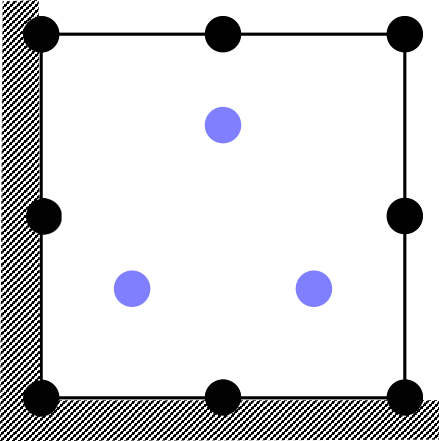
\includegraphics[width=0.3\textwidth]{figures/Q8P3.png} &
            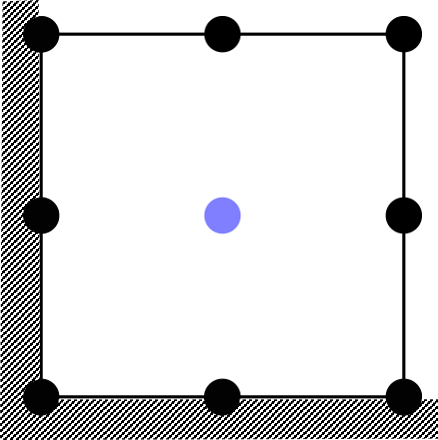
\includegraphics[width=0.3\textwidth]{figures/Q8P1.png} \\
            (a) & (b) \\
            \raisebox{-0.3\height}{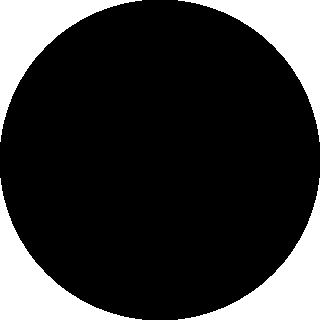
\includegraphics[width=14pt]{figures/legend_u.png}} :位移节点 &
            \raisebox{-0.3\height}{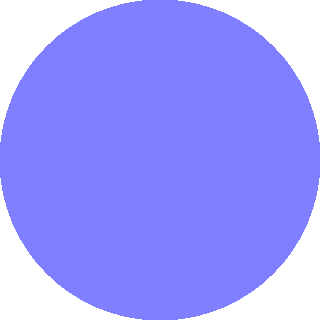
\includegraphics[width=14pt]{figures/legend_p.png}} :压力节点 
        \end{tabular}
        \caption{二维位移压力单元示例}\label{ch_3:fig:elements_eg}
    \end{figure}

表\ref{ch_3:tab:infsup2}为其他经典单元的验证结果,通过对比分析可以看出,本文所提的验证LBB稳定性条件的新方法,其验证结果与数值验证方法和解析证明方法完全一致。这一结果表明,新方法在使用简易的同时,能够有效的验证混合离散方案的LBB稳定性条件。
\begin{table}[!h]
    \centering
    \renewcommand\arraystretch{1.2}
    \caption{inf-sup条件验证} \label{ch_3:tab:infsup2}
    \begin{tabular}{ccccc}
        \hline
        \multirow{2}{*}{离散方案}&体积&\multicolumn{3}{c}{inf-sup条件}\\
        & 约束比&数值验证&解析证明&系数估计\\
        \hline
        \begin{tabular}{c}
            \begin{minipage}{0.1\columnwidth}
                \centering
                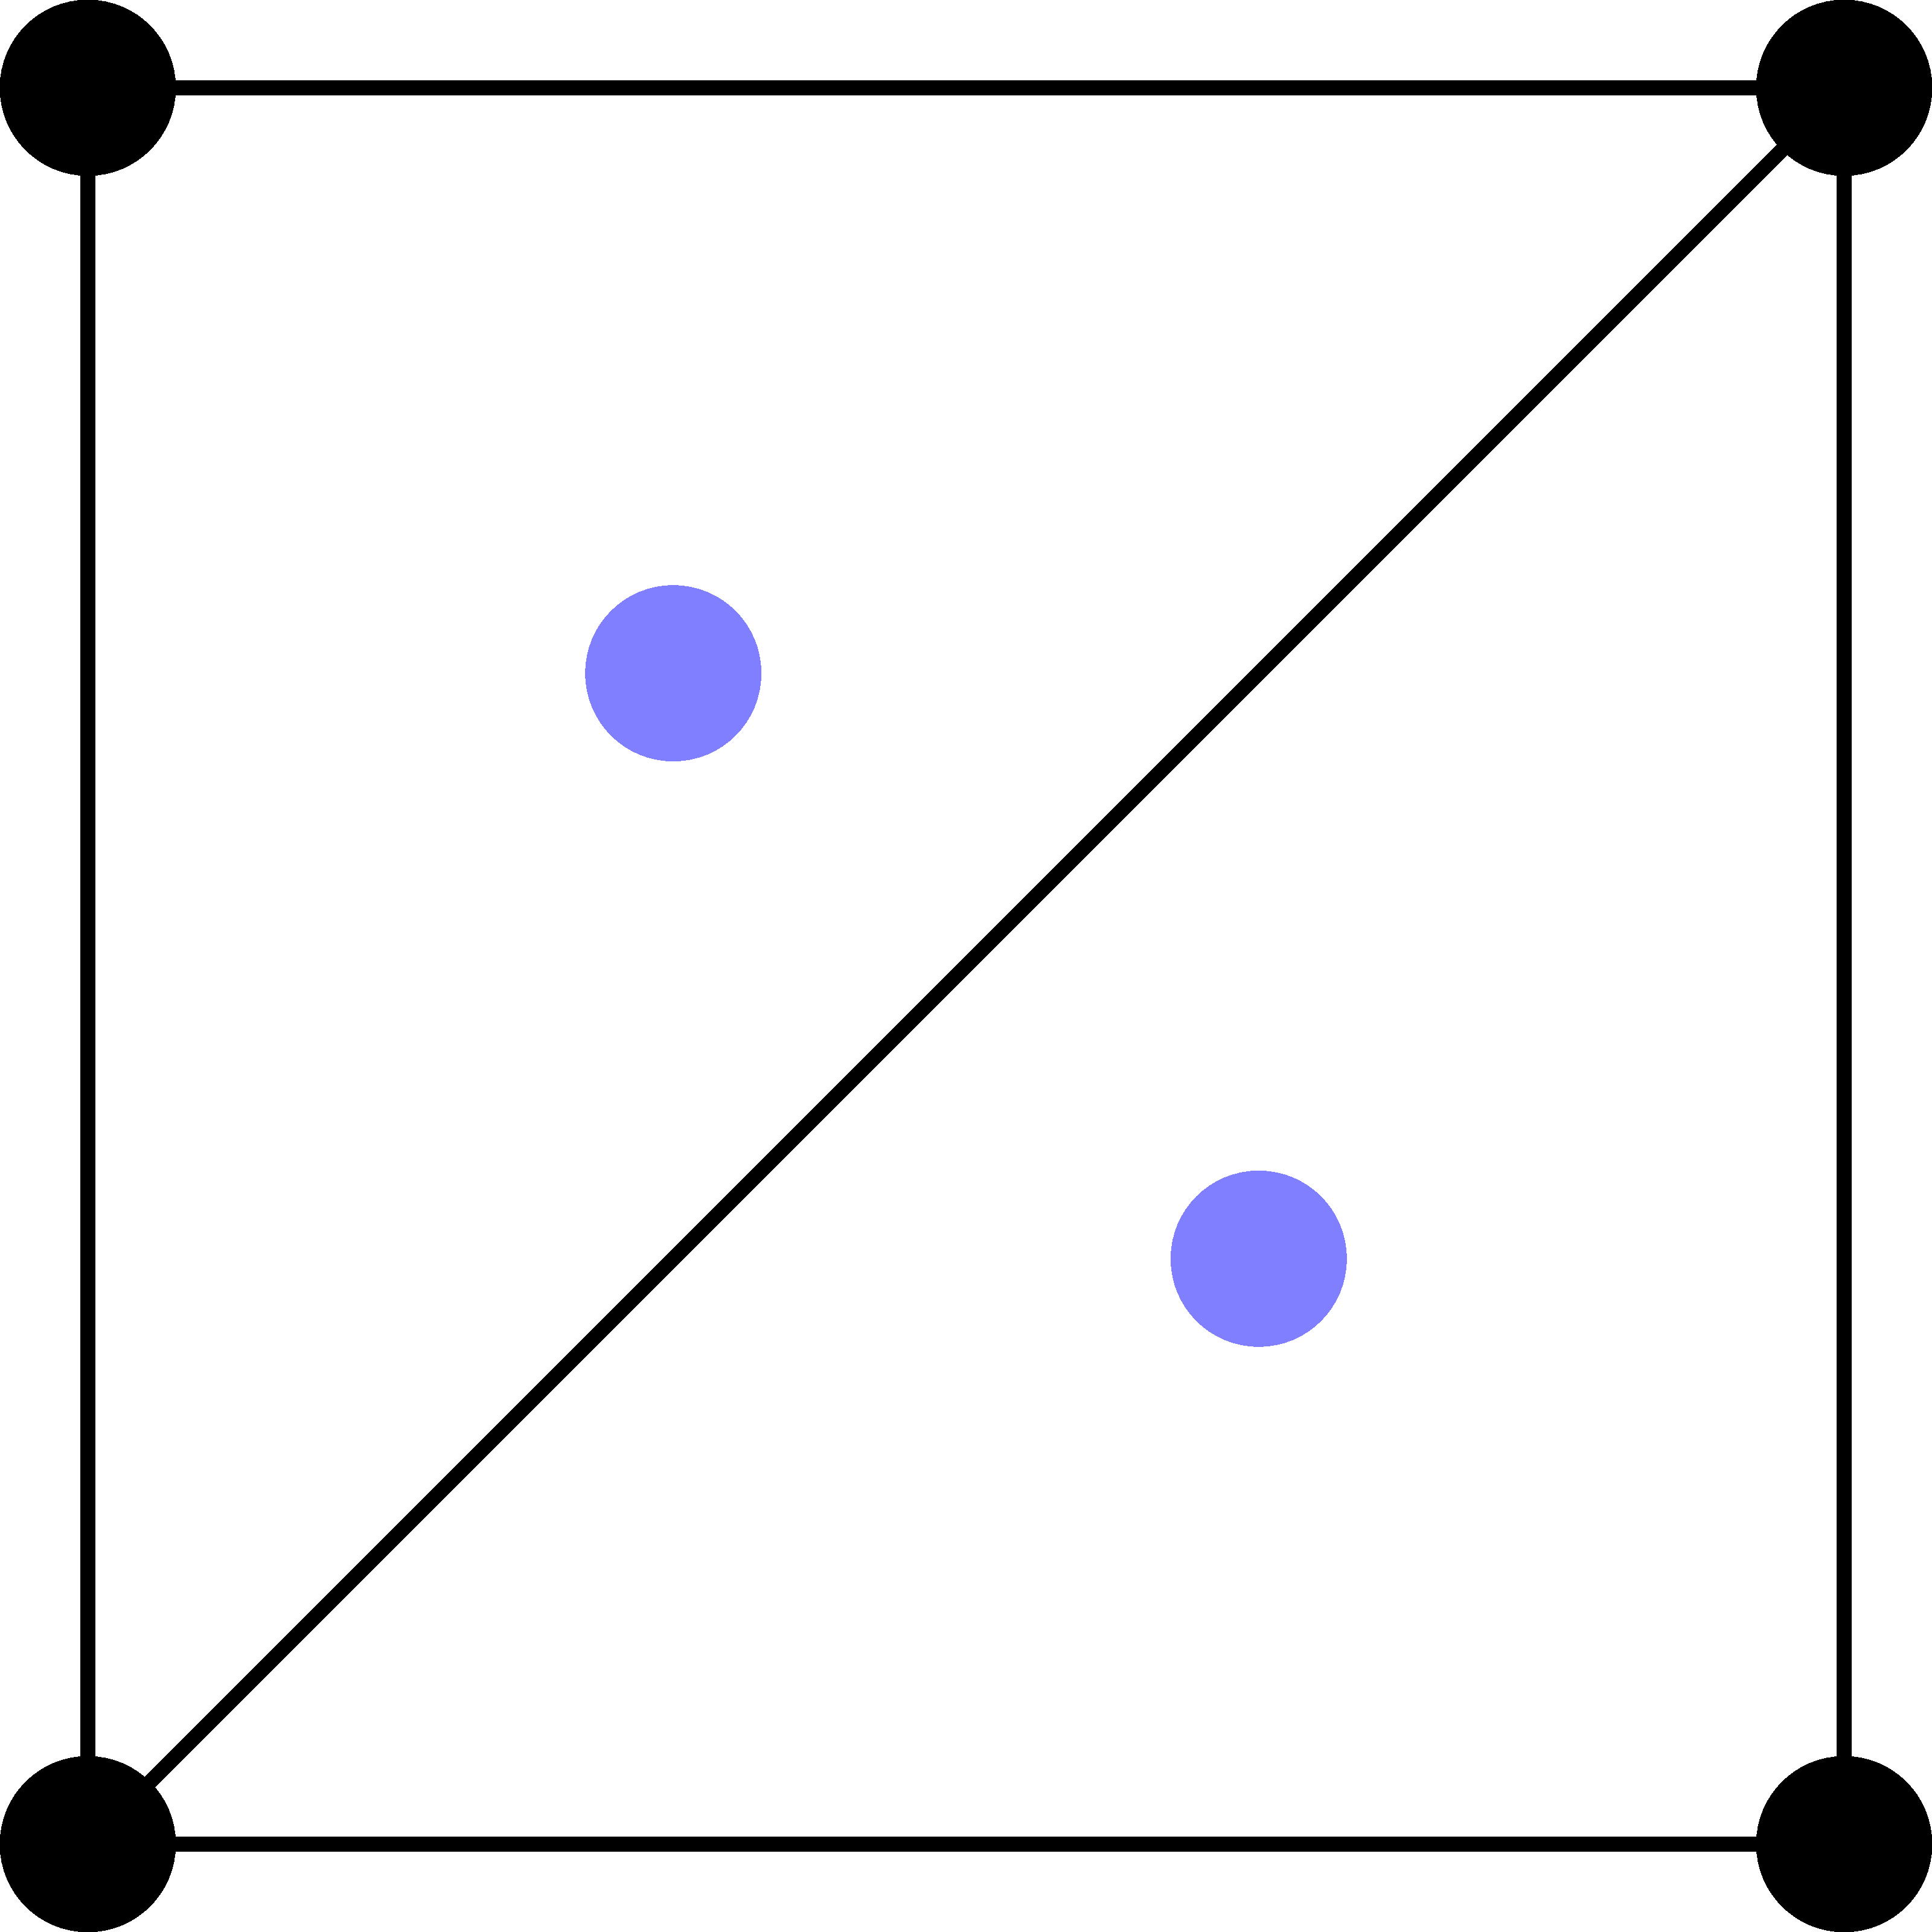
\includegraphics[width=0.9\textwidth]{figures/mix_T3P1.png}
            \end{minipage}\\T3P1
        \end{tabular}
        &1&$\times$ & $\times$&$\times$\\
        \begin{tabular}{c}
            \begin{minipage}{0.1\columnwidth}
                \centering
                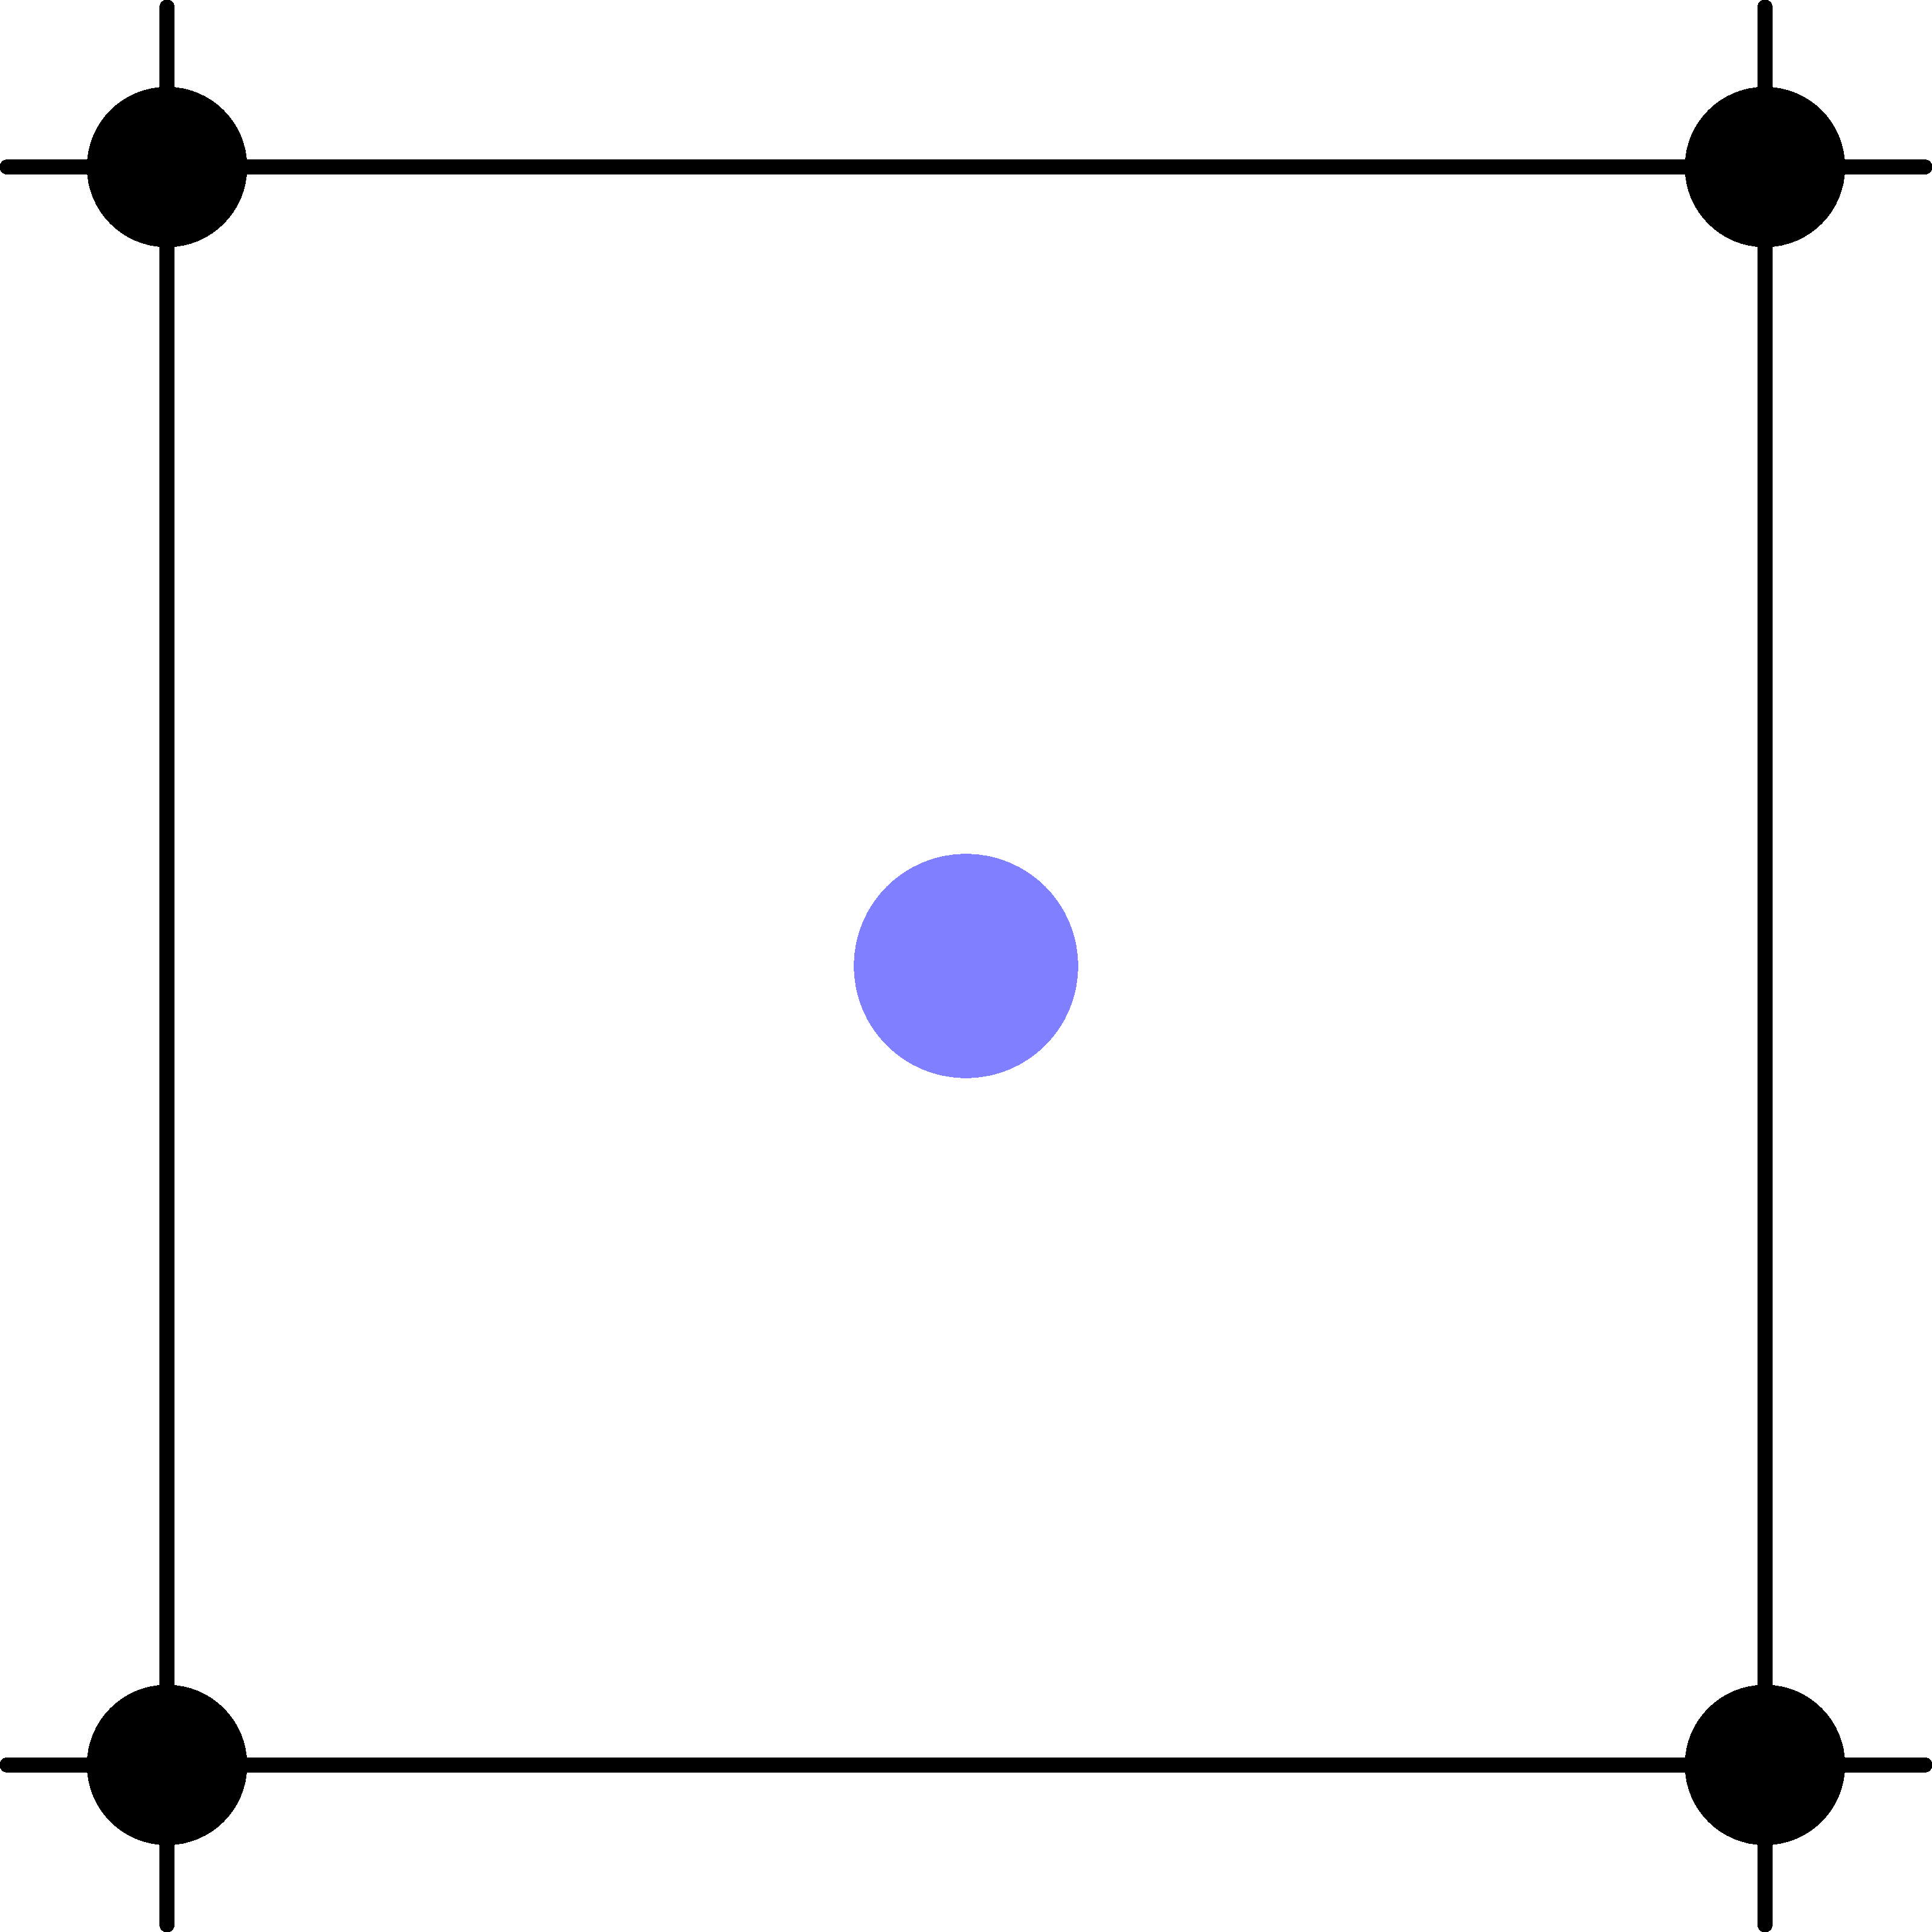
\includegraphics[width=0.9\textwidth]{figures/mix_Q4P1.png}
            \end{minipage}\\Q4P1
        \end{tabular}
        &2&$\times$ & $\times$&$\times$\\
        \begin{tabular}{c}
            \begin{minipage}{0.1\columnwidth}
                \centering
                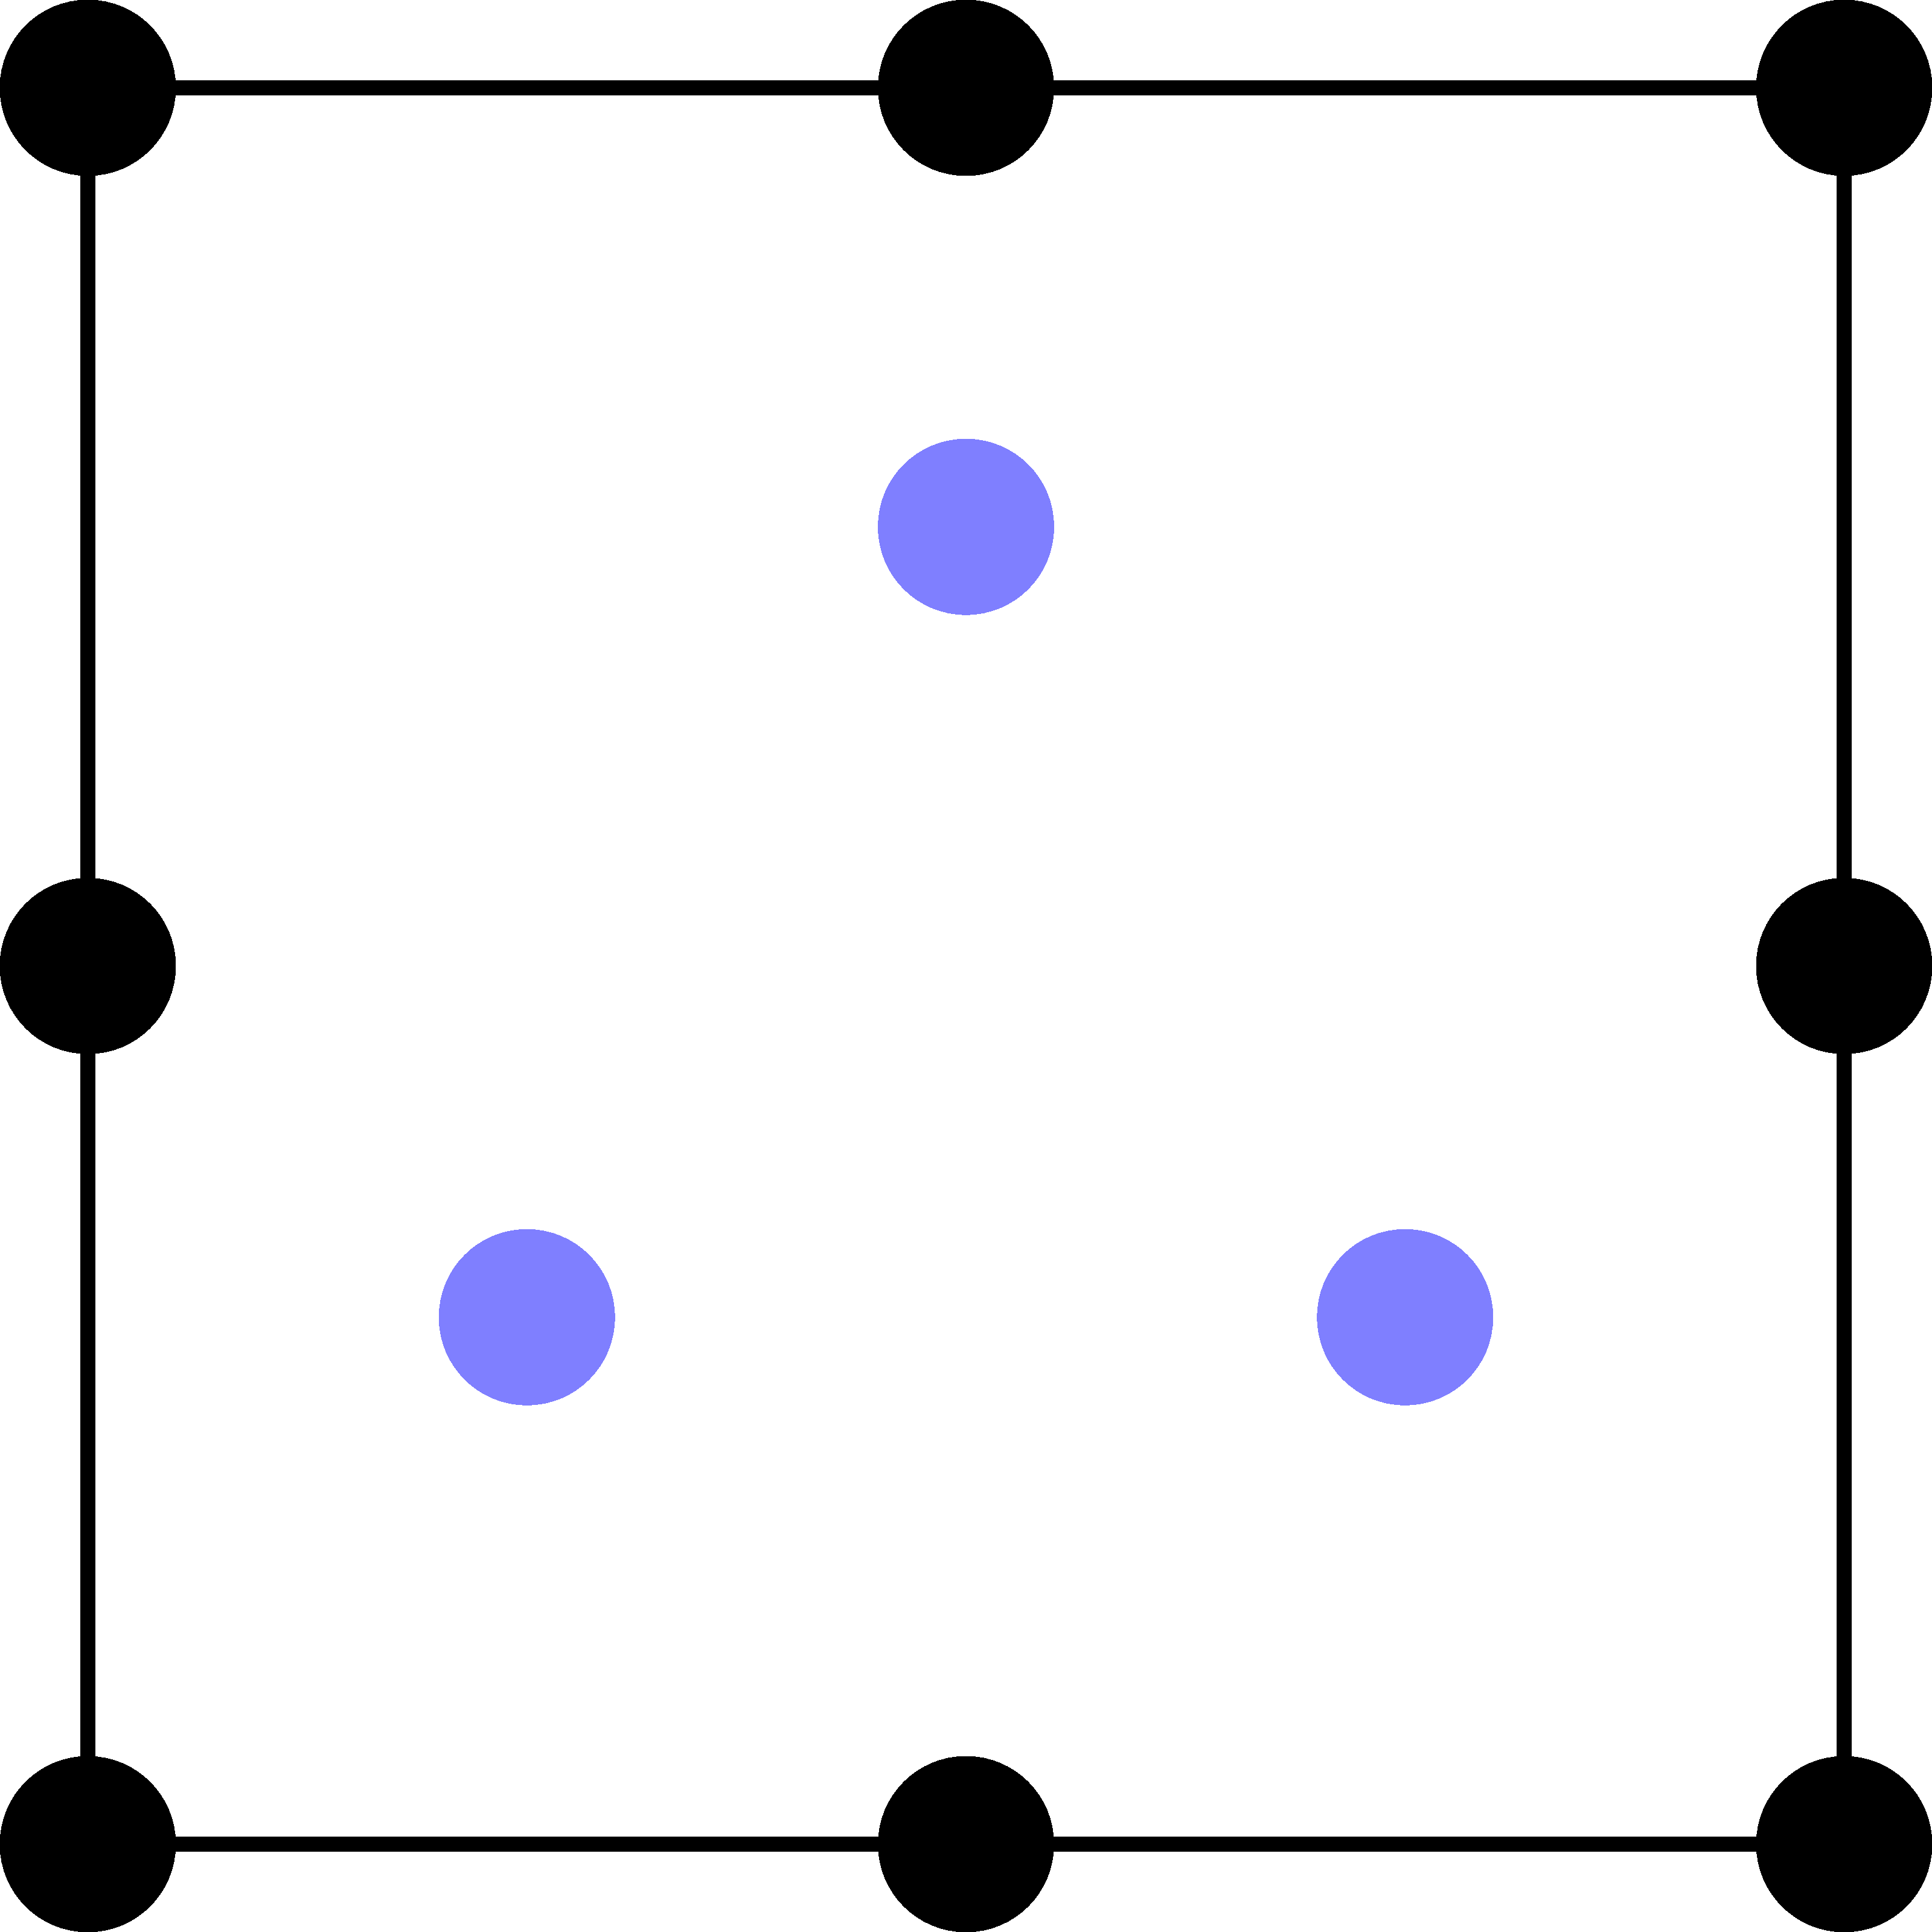
\includegraphics[width=0.9\textwidth]{figures/mix_Q8P3.png}
            \end{minipage}\\Q8P3
        \end{tabular}
        &2&$\times$ & $\times$&$\times$\\
        \begin{tabular}{c}
            \begin{minipage}{0.1\columnwidth}
                \centering
                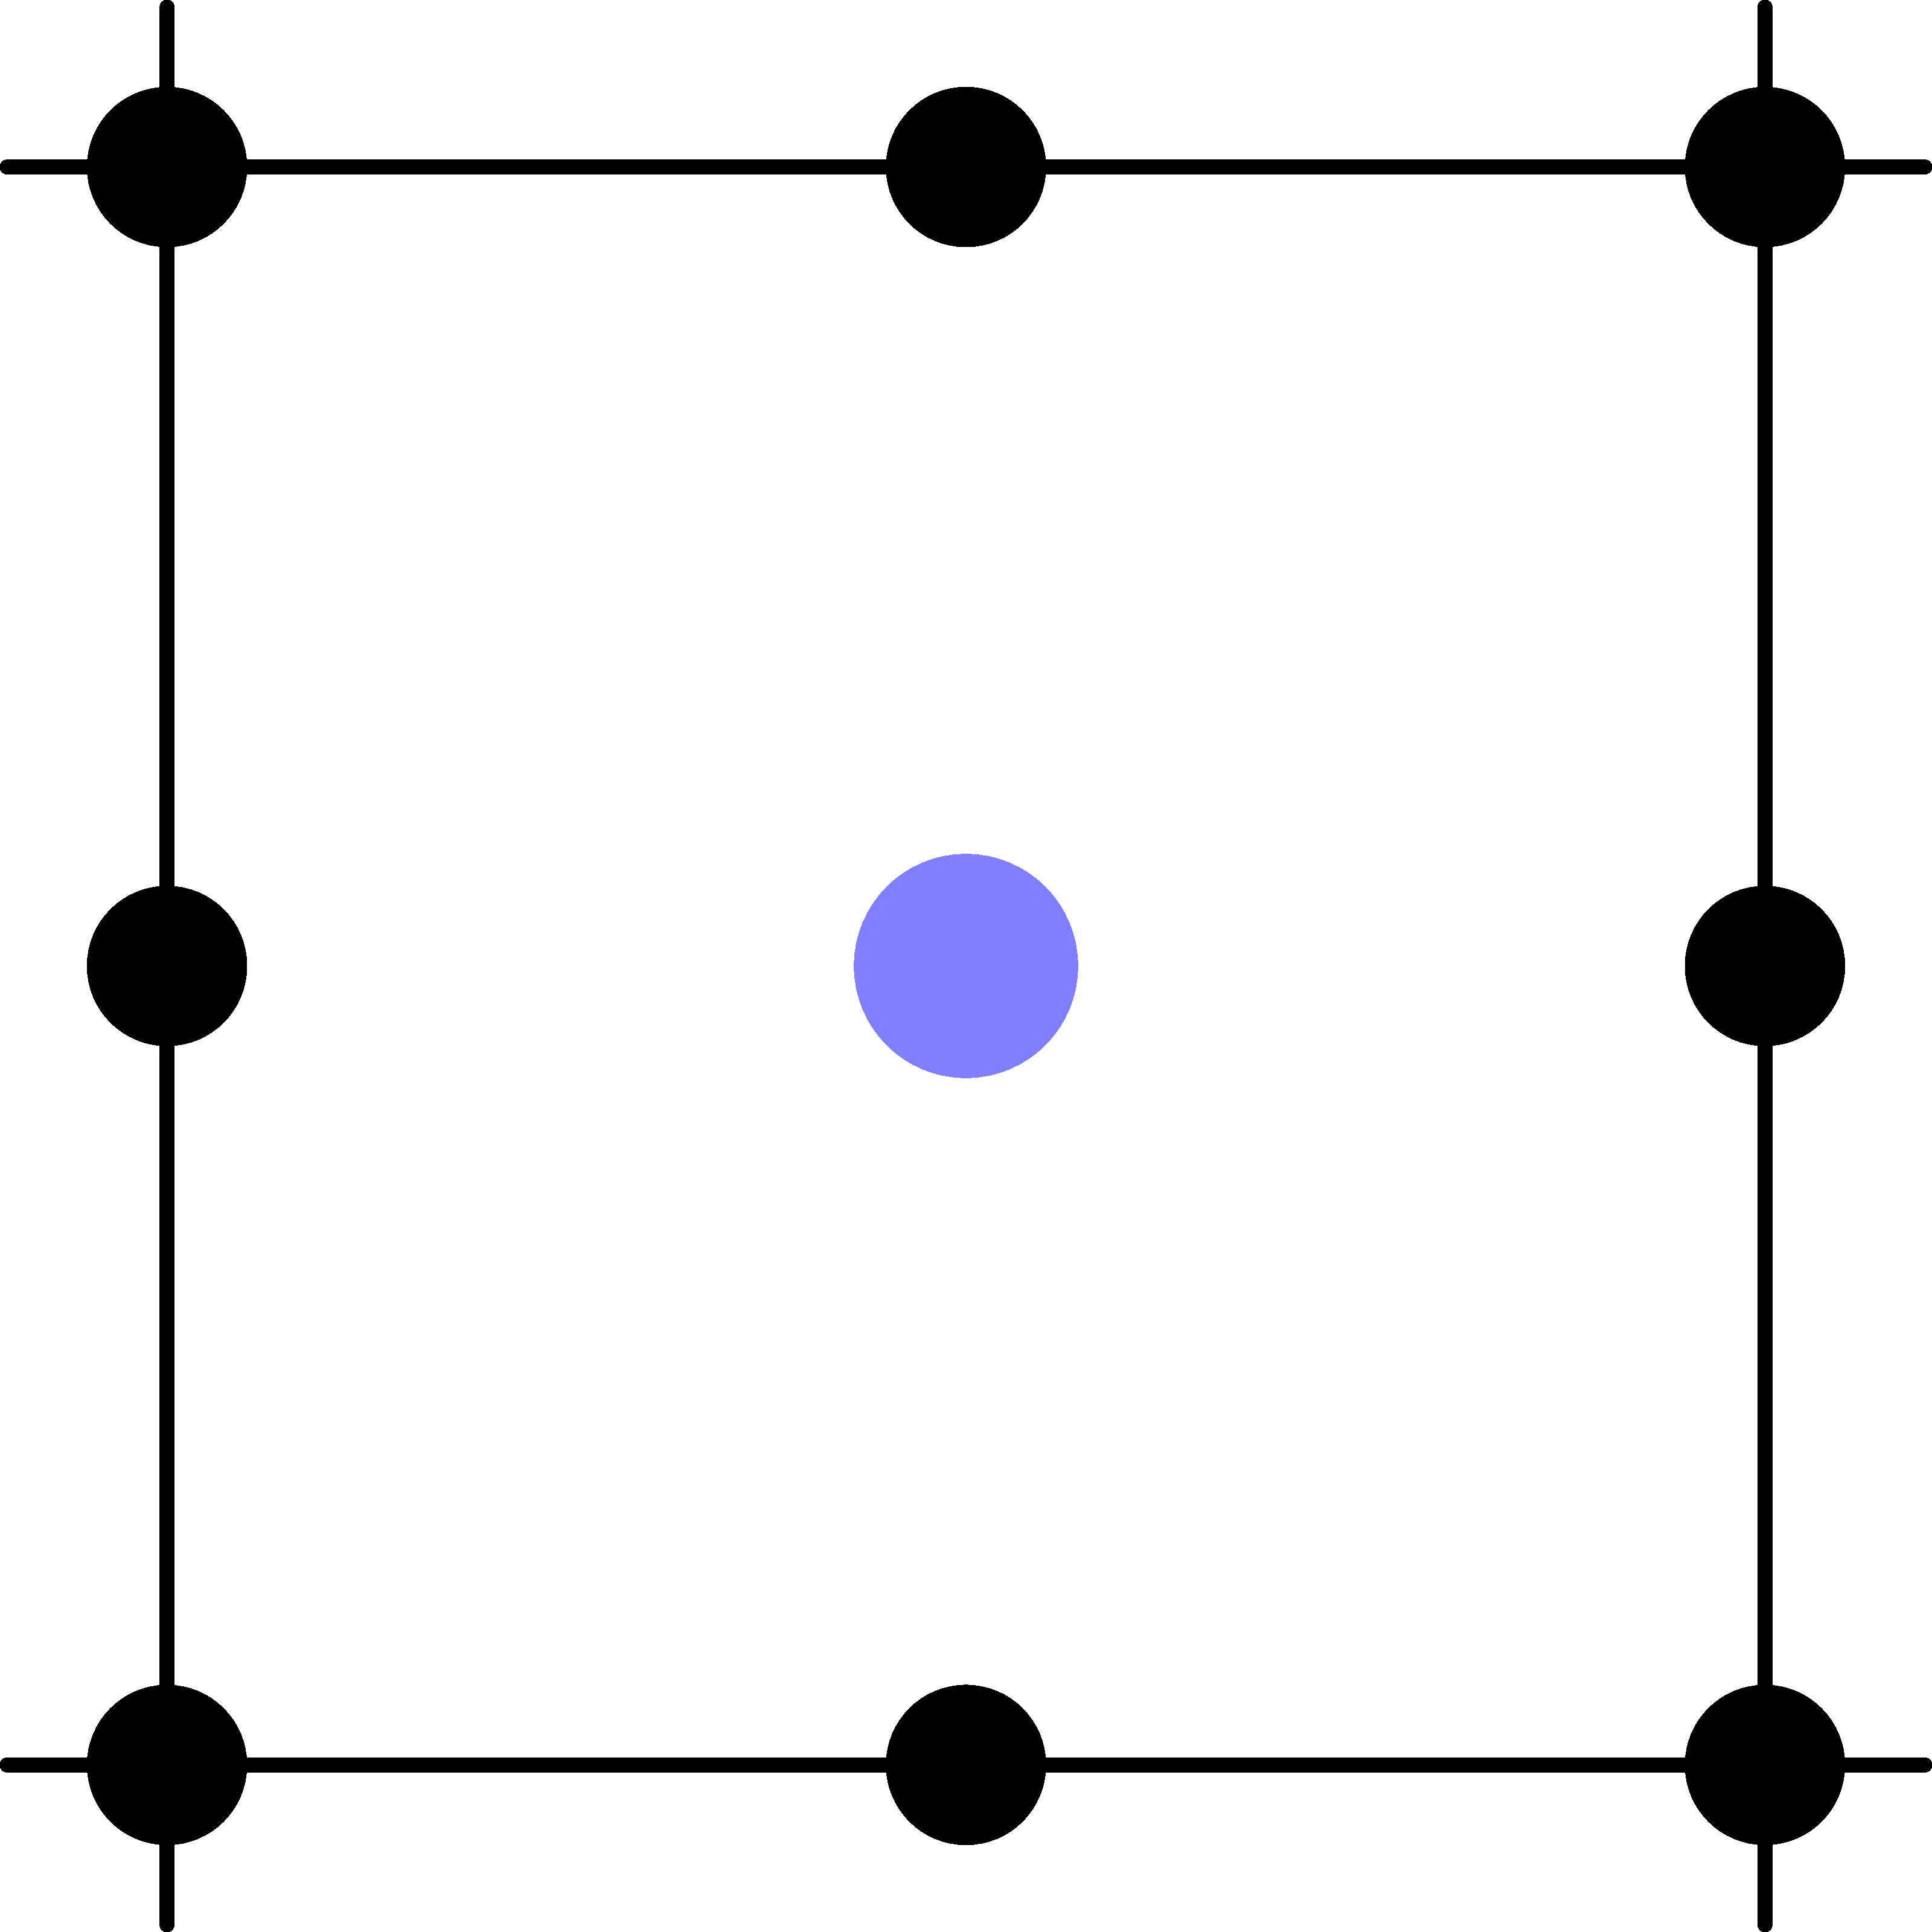
\includegraphics[width=0.9\textwidth]{figures/mix_Q8P1.png}
            \end{minipage}\\Q8P1
        \end{tabular}
        &6&\checkmark & \checkmark & \checkmark\\
        \begin{tabular}{c}
            \begin{minipage}{0.1\columnwidth}
                \centering
                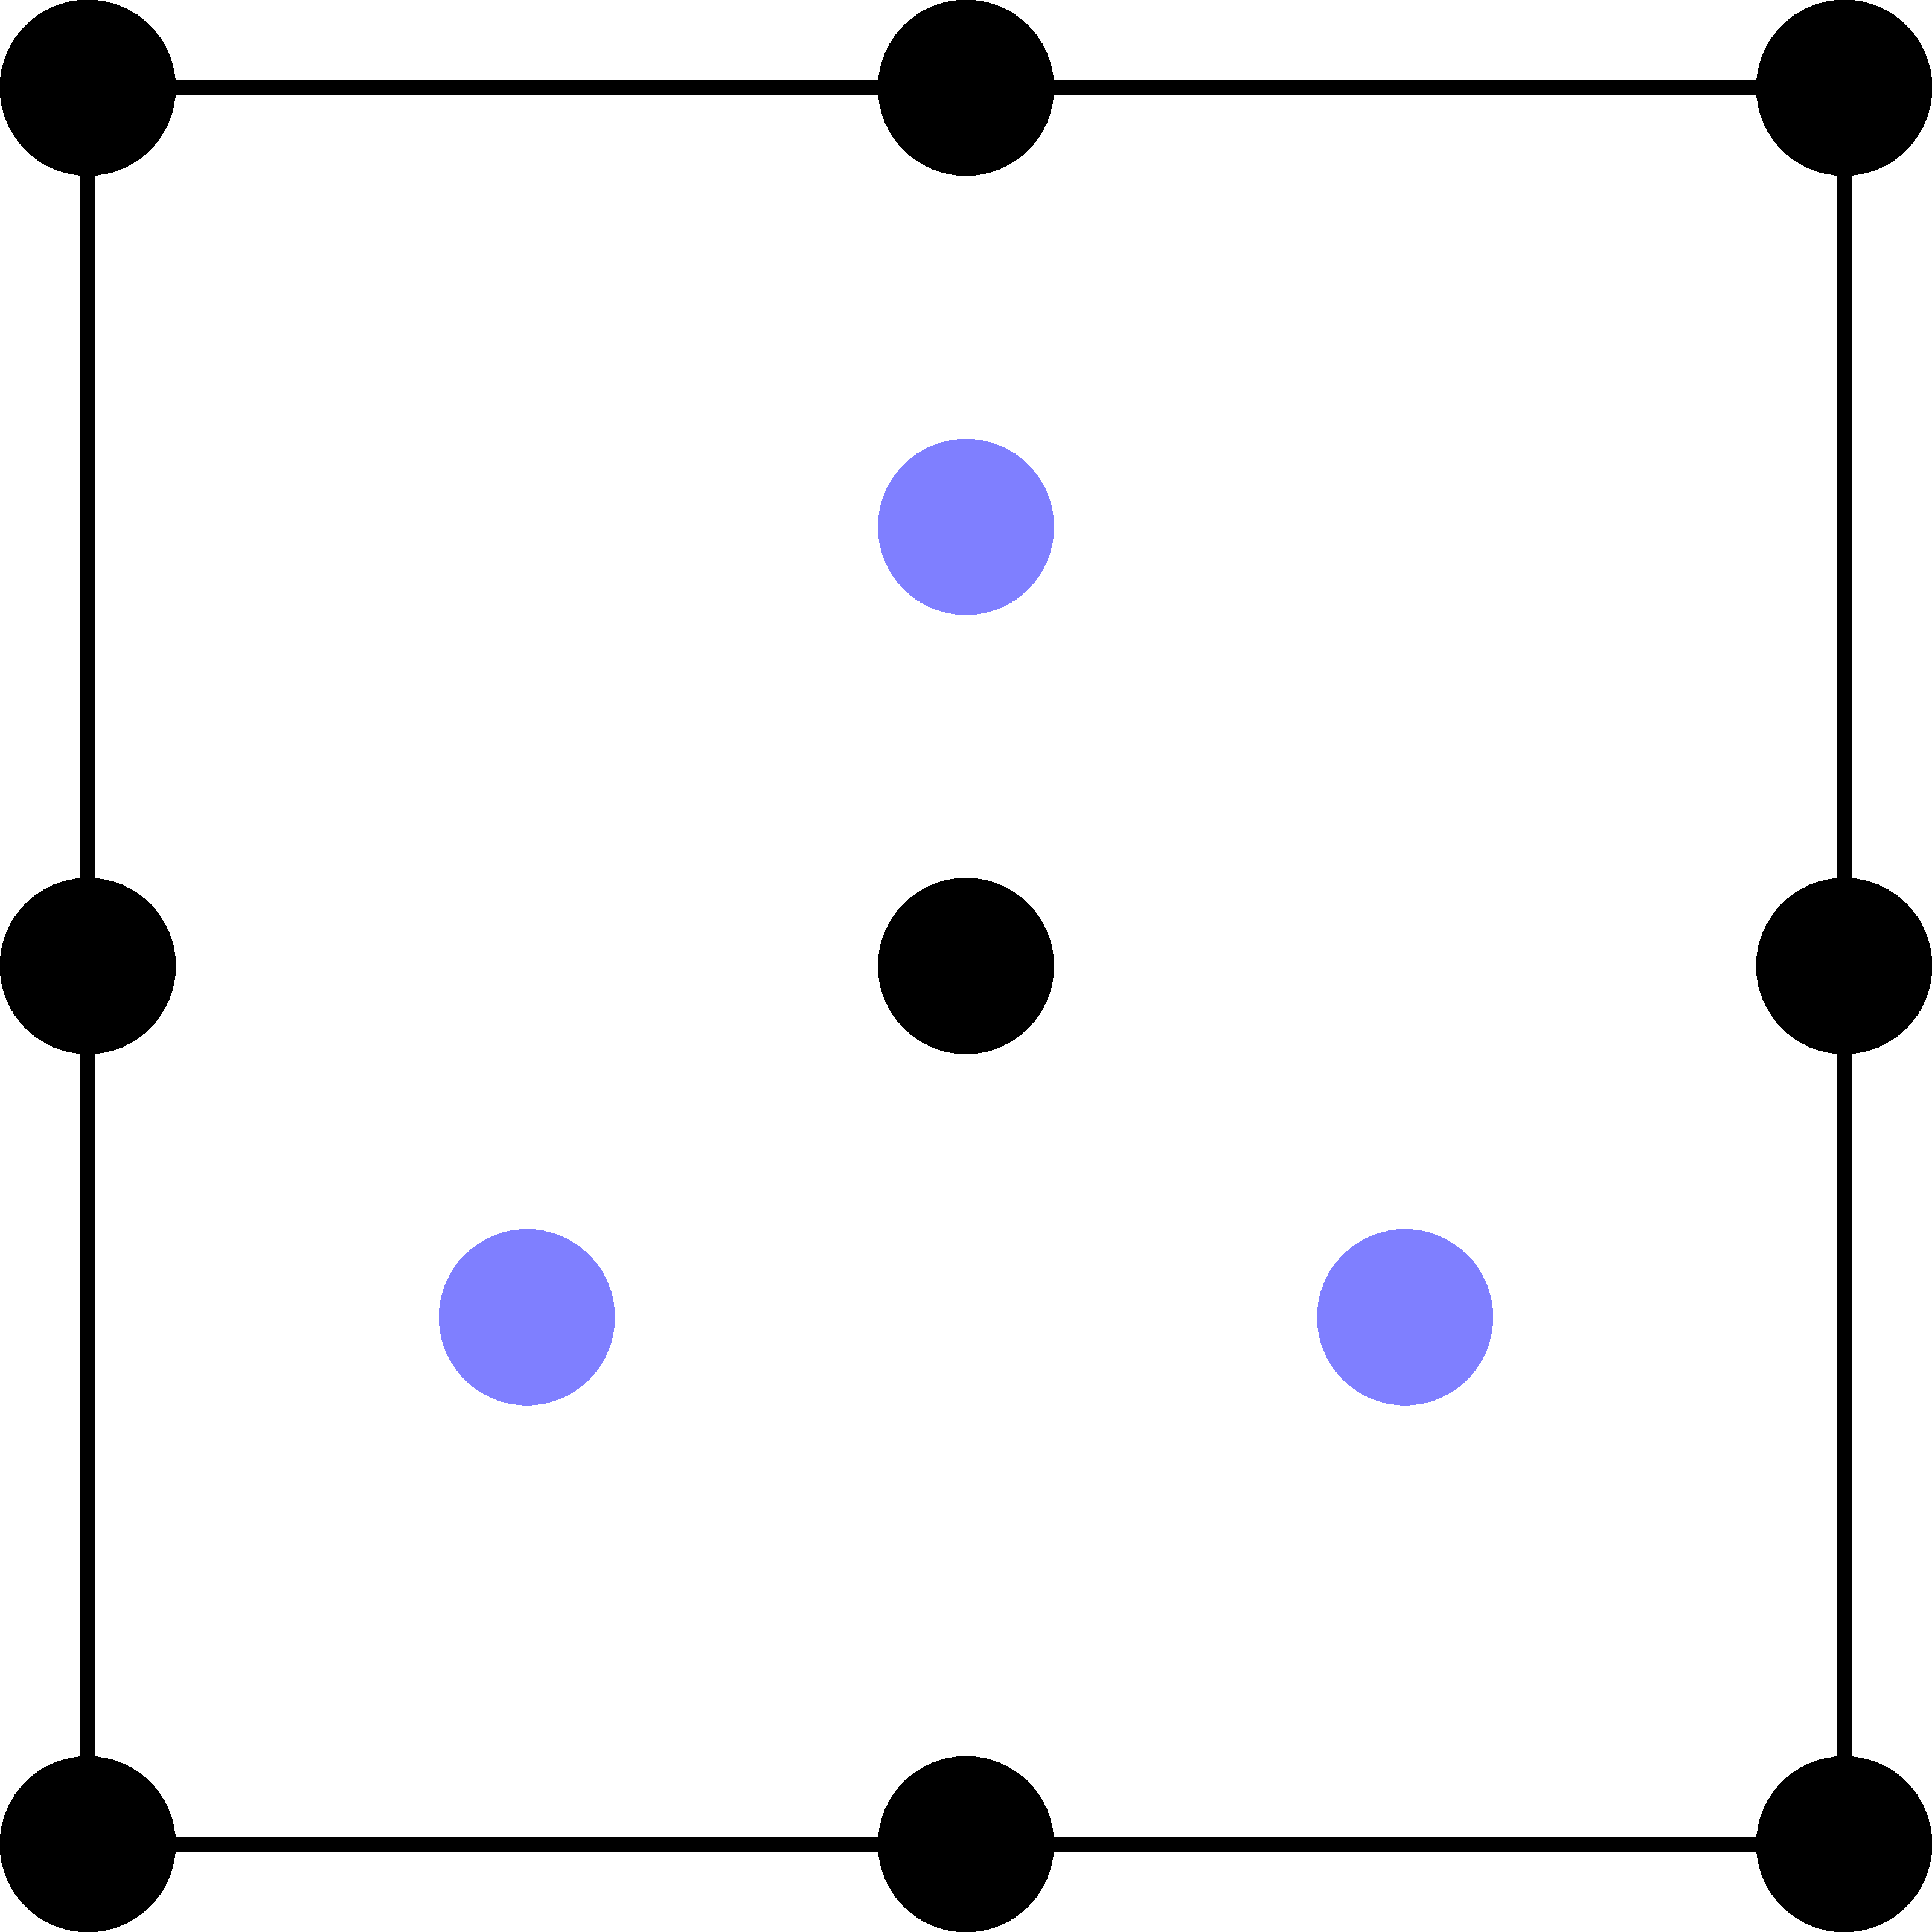
\includegraphics[width=0.9\textwidth]{figures/mix_Q9P3.png}
            \end{minipage}\\Q9P3
        \end{tabular}
        &$\frac{8}{3}$&\checkmark & \checkmark & \checkmark\\
        \begin{tabular}{c}
            \begin{minipage}{0.1\columnwidth}
                \centering
                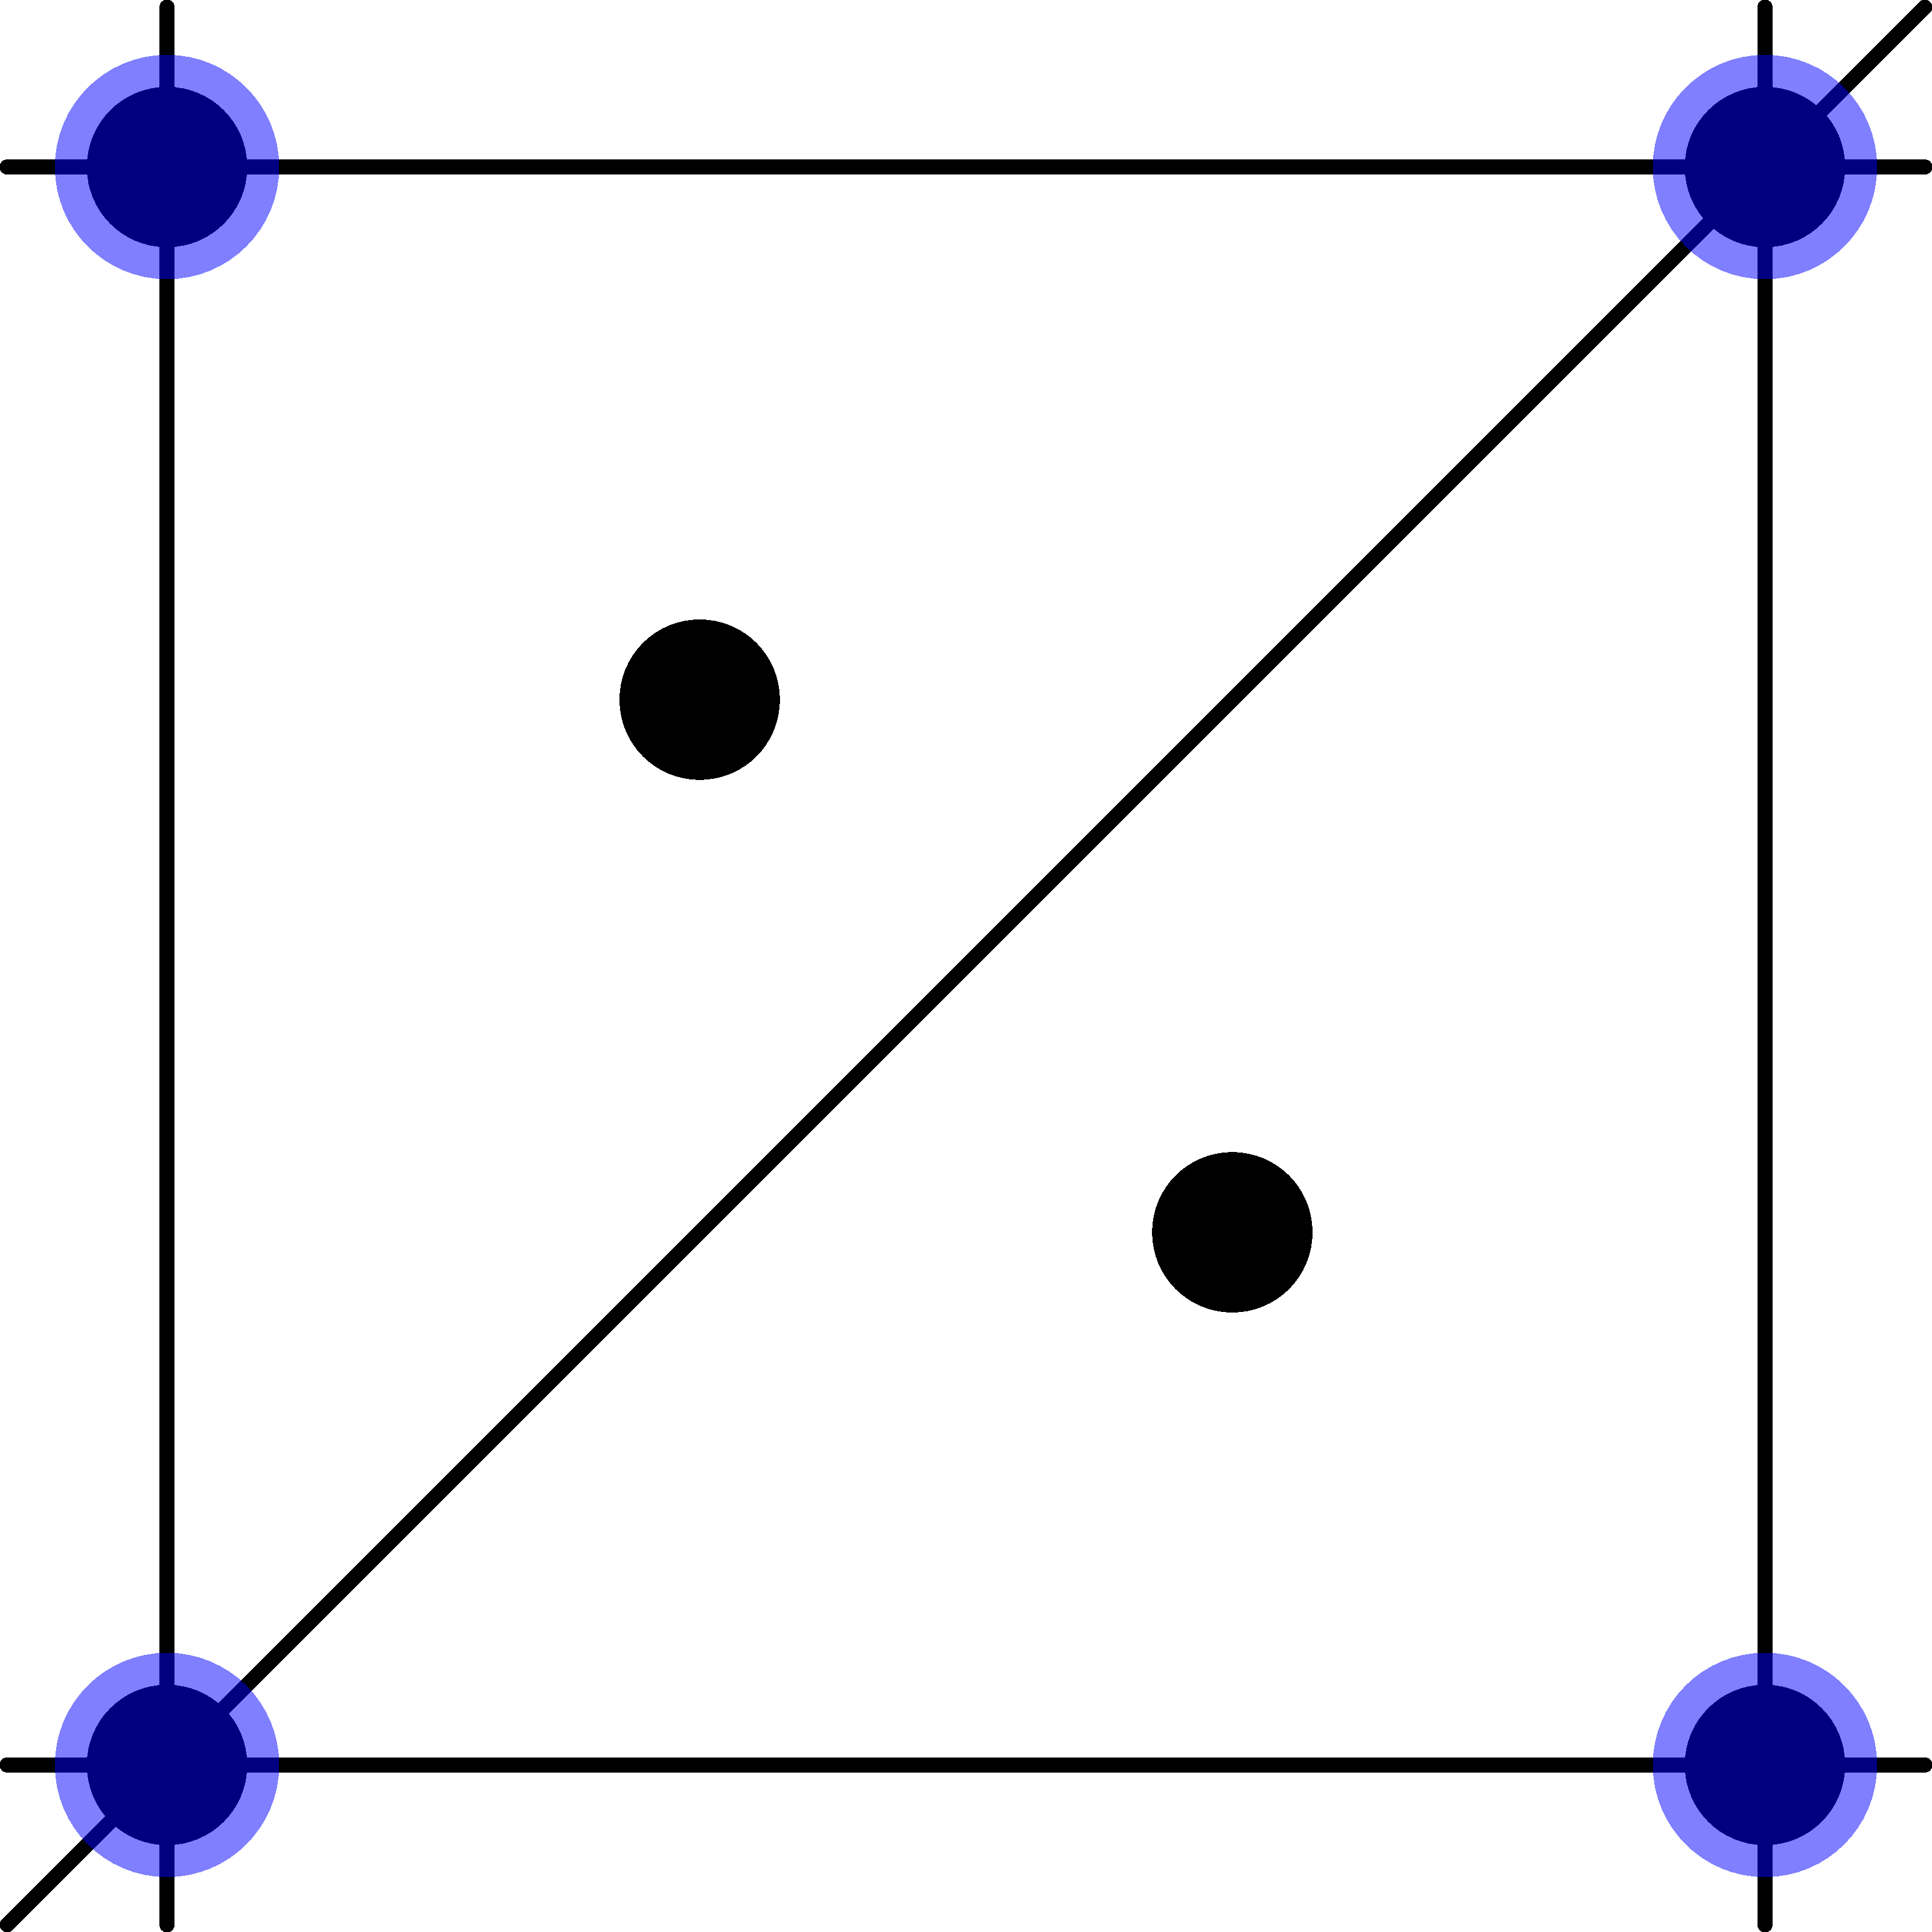
\includegraphics[width=0.9\textwidth]{figures/mini.png}
            \end{minipage}\\MINI element \cite{arnold1984,auricchio2005}
        \end{tabular}
        &$\frac{8}{3}$&\checkmark & \checkmark& \checkmark\\
        \begin{tabular}{c}
            \begin{minipage}{0.1\columnwidth}
                \centering
                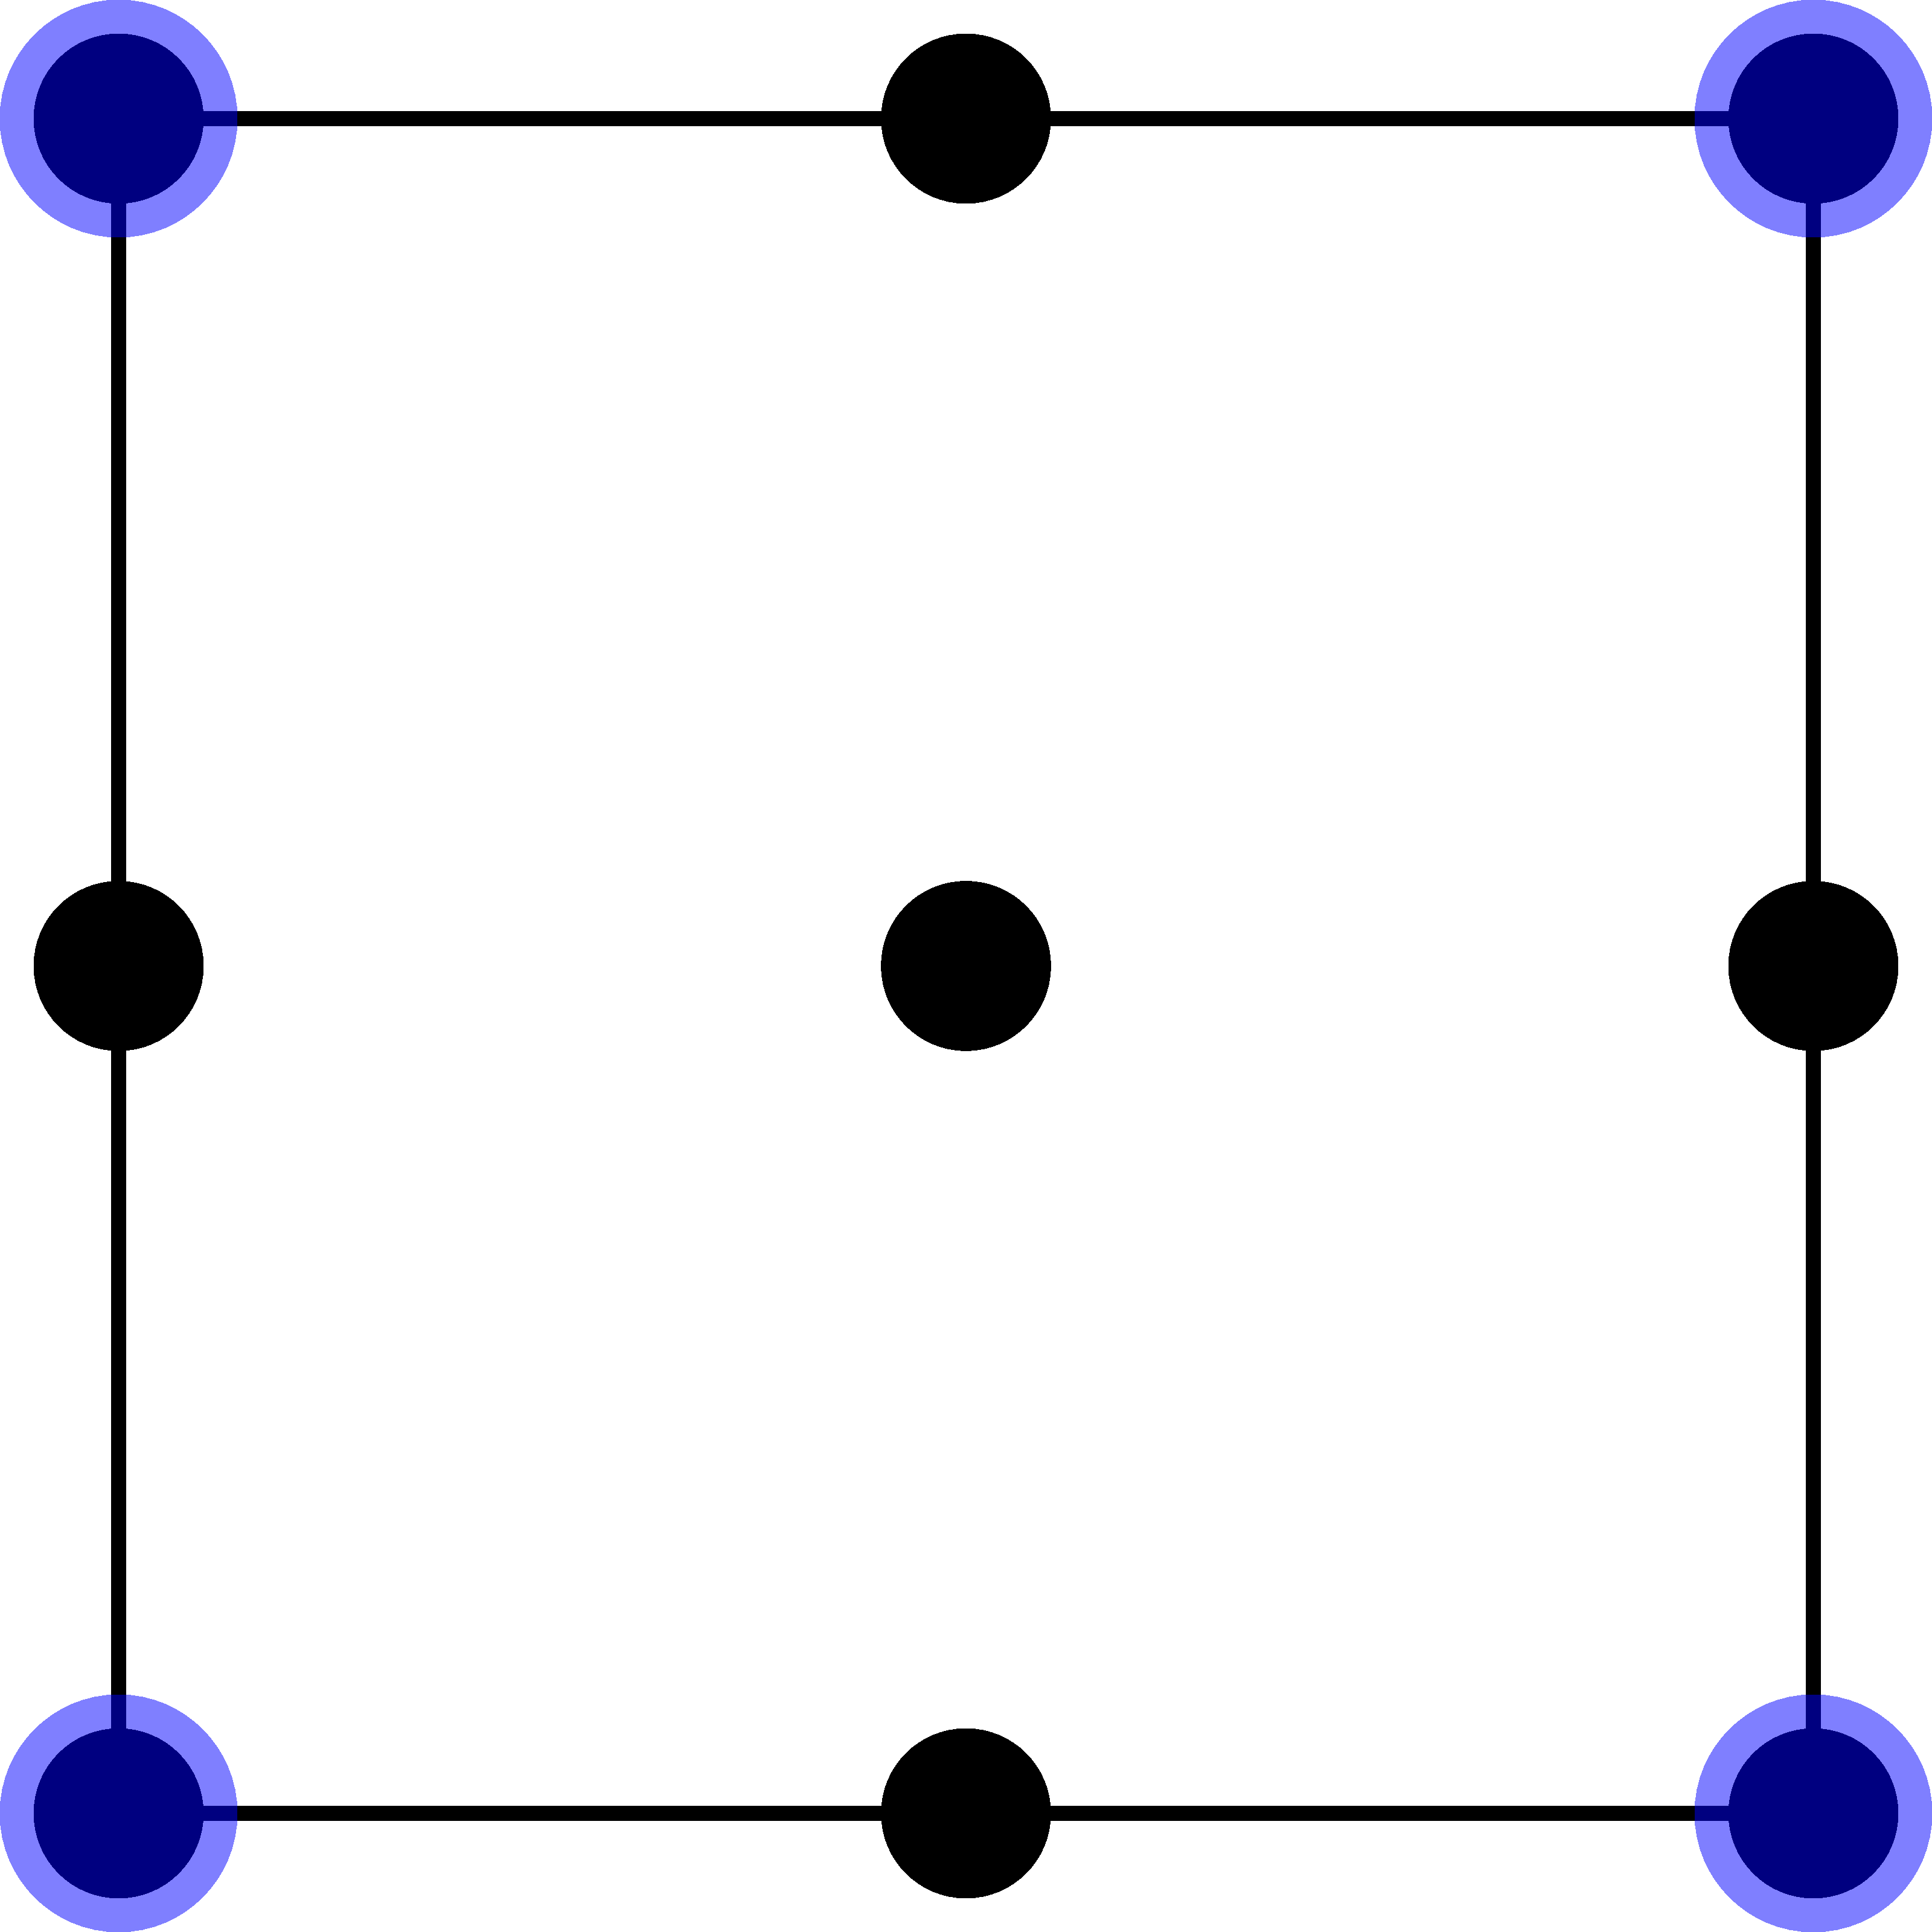
\includegraphics[width=0.9\textwidth]{figures/TaylorHood.png}
            \end{minipage}\\Taylor--Hood element \cite{hood1974}
        \end{tabular}
        &$\frac{8}{3}$&\checkmark & \checkmark& \checkmark\\
        \begin{tabular}{c}
            \begin{minipage}{0.1\columnwidth}
                \centering
                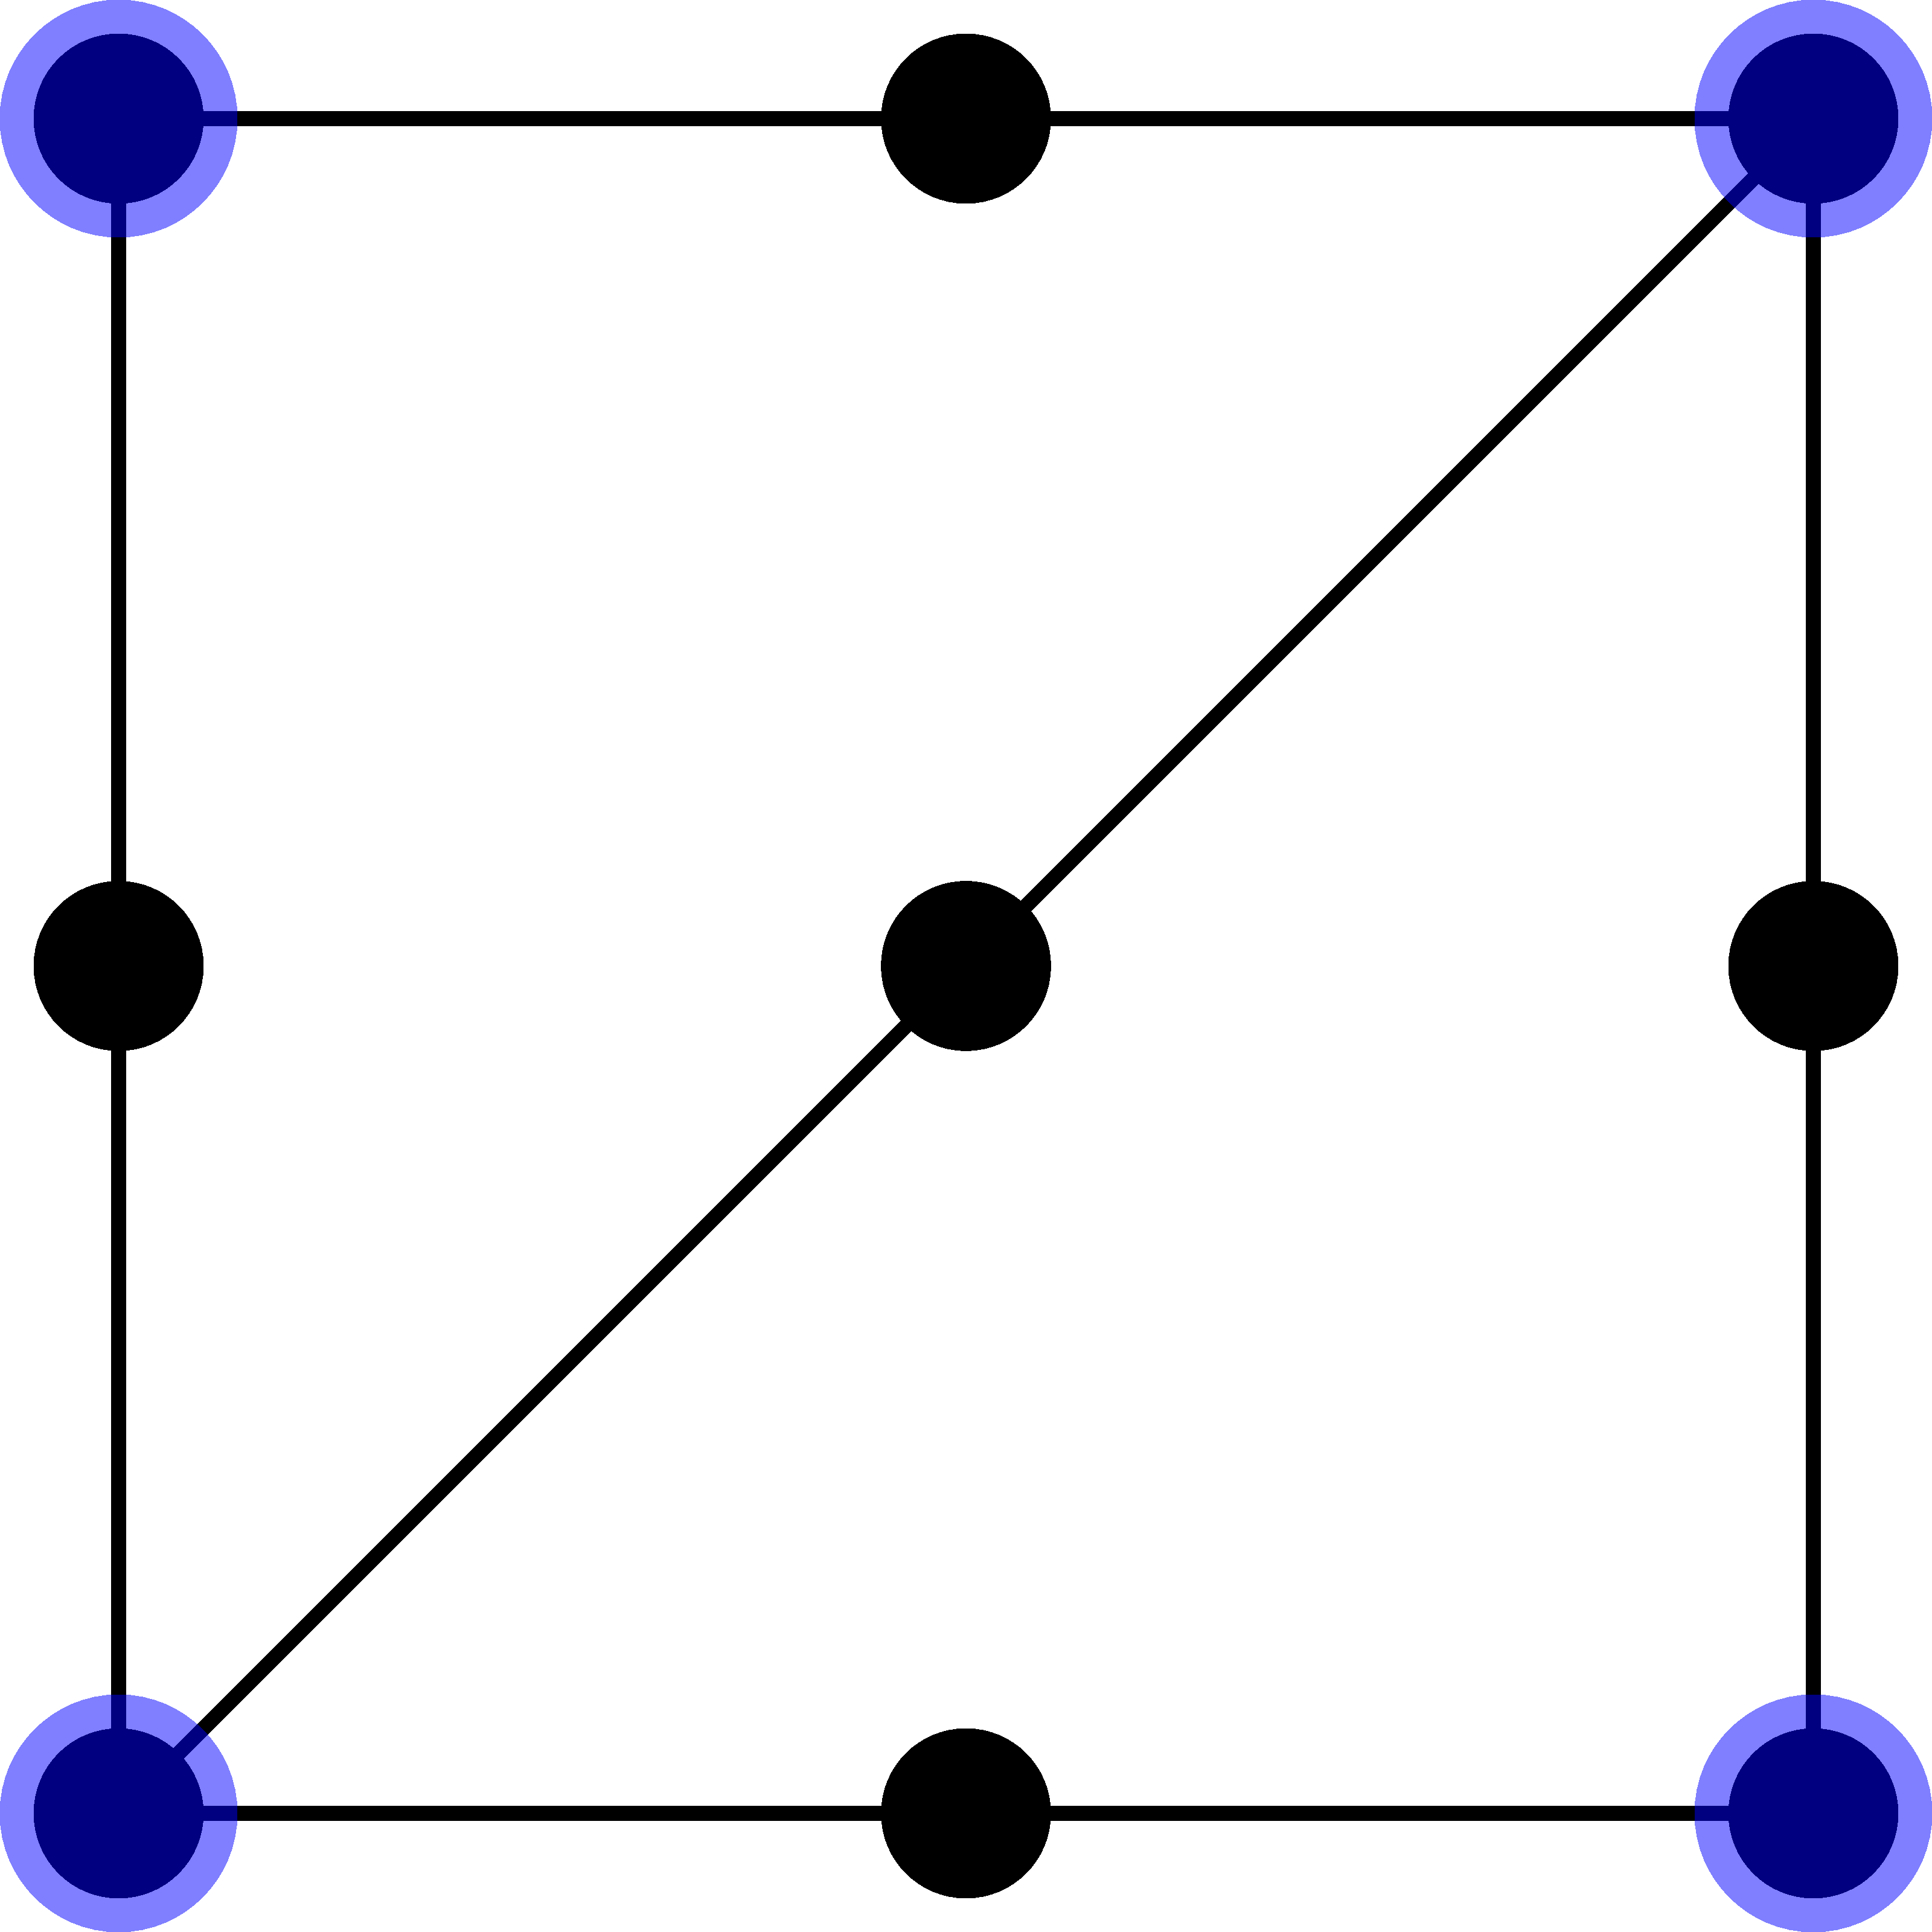
\includegraphics[width=0.9\textwidth]{figures/mix_T6C3.png}
            \end{minipage}\\T6C3
        \end{tabular}
        &8&\checkmark & & \checkmark\\
        \begin{tabular}{c}
            \begin{minipage}{0.1\columnwidth}
                \centering
                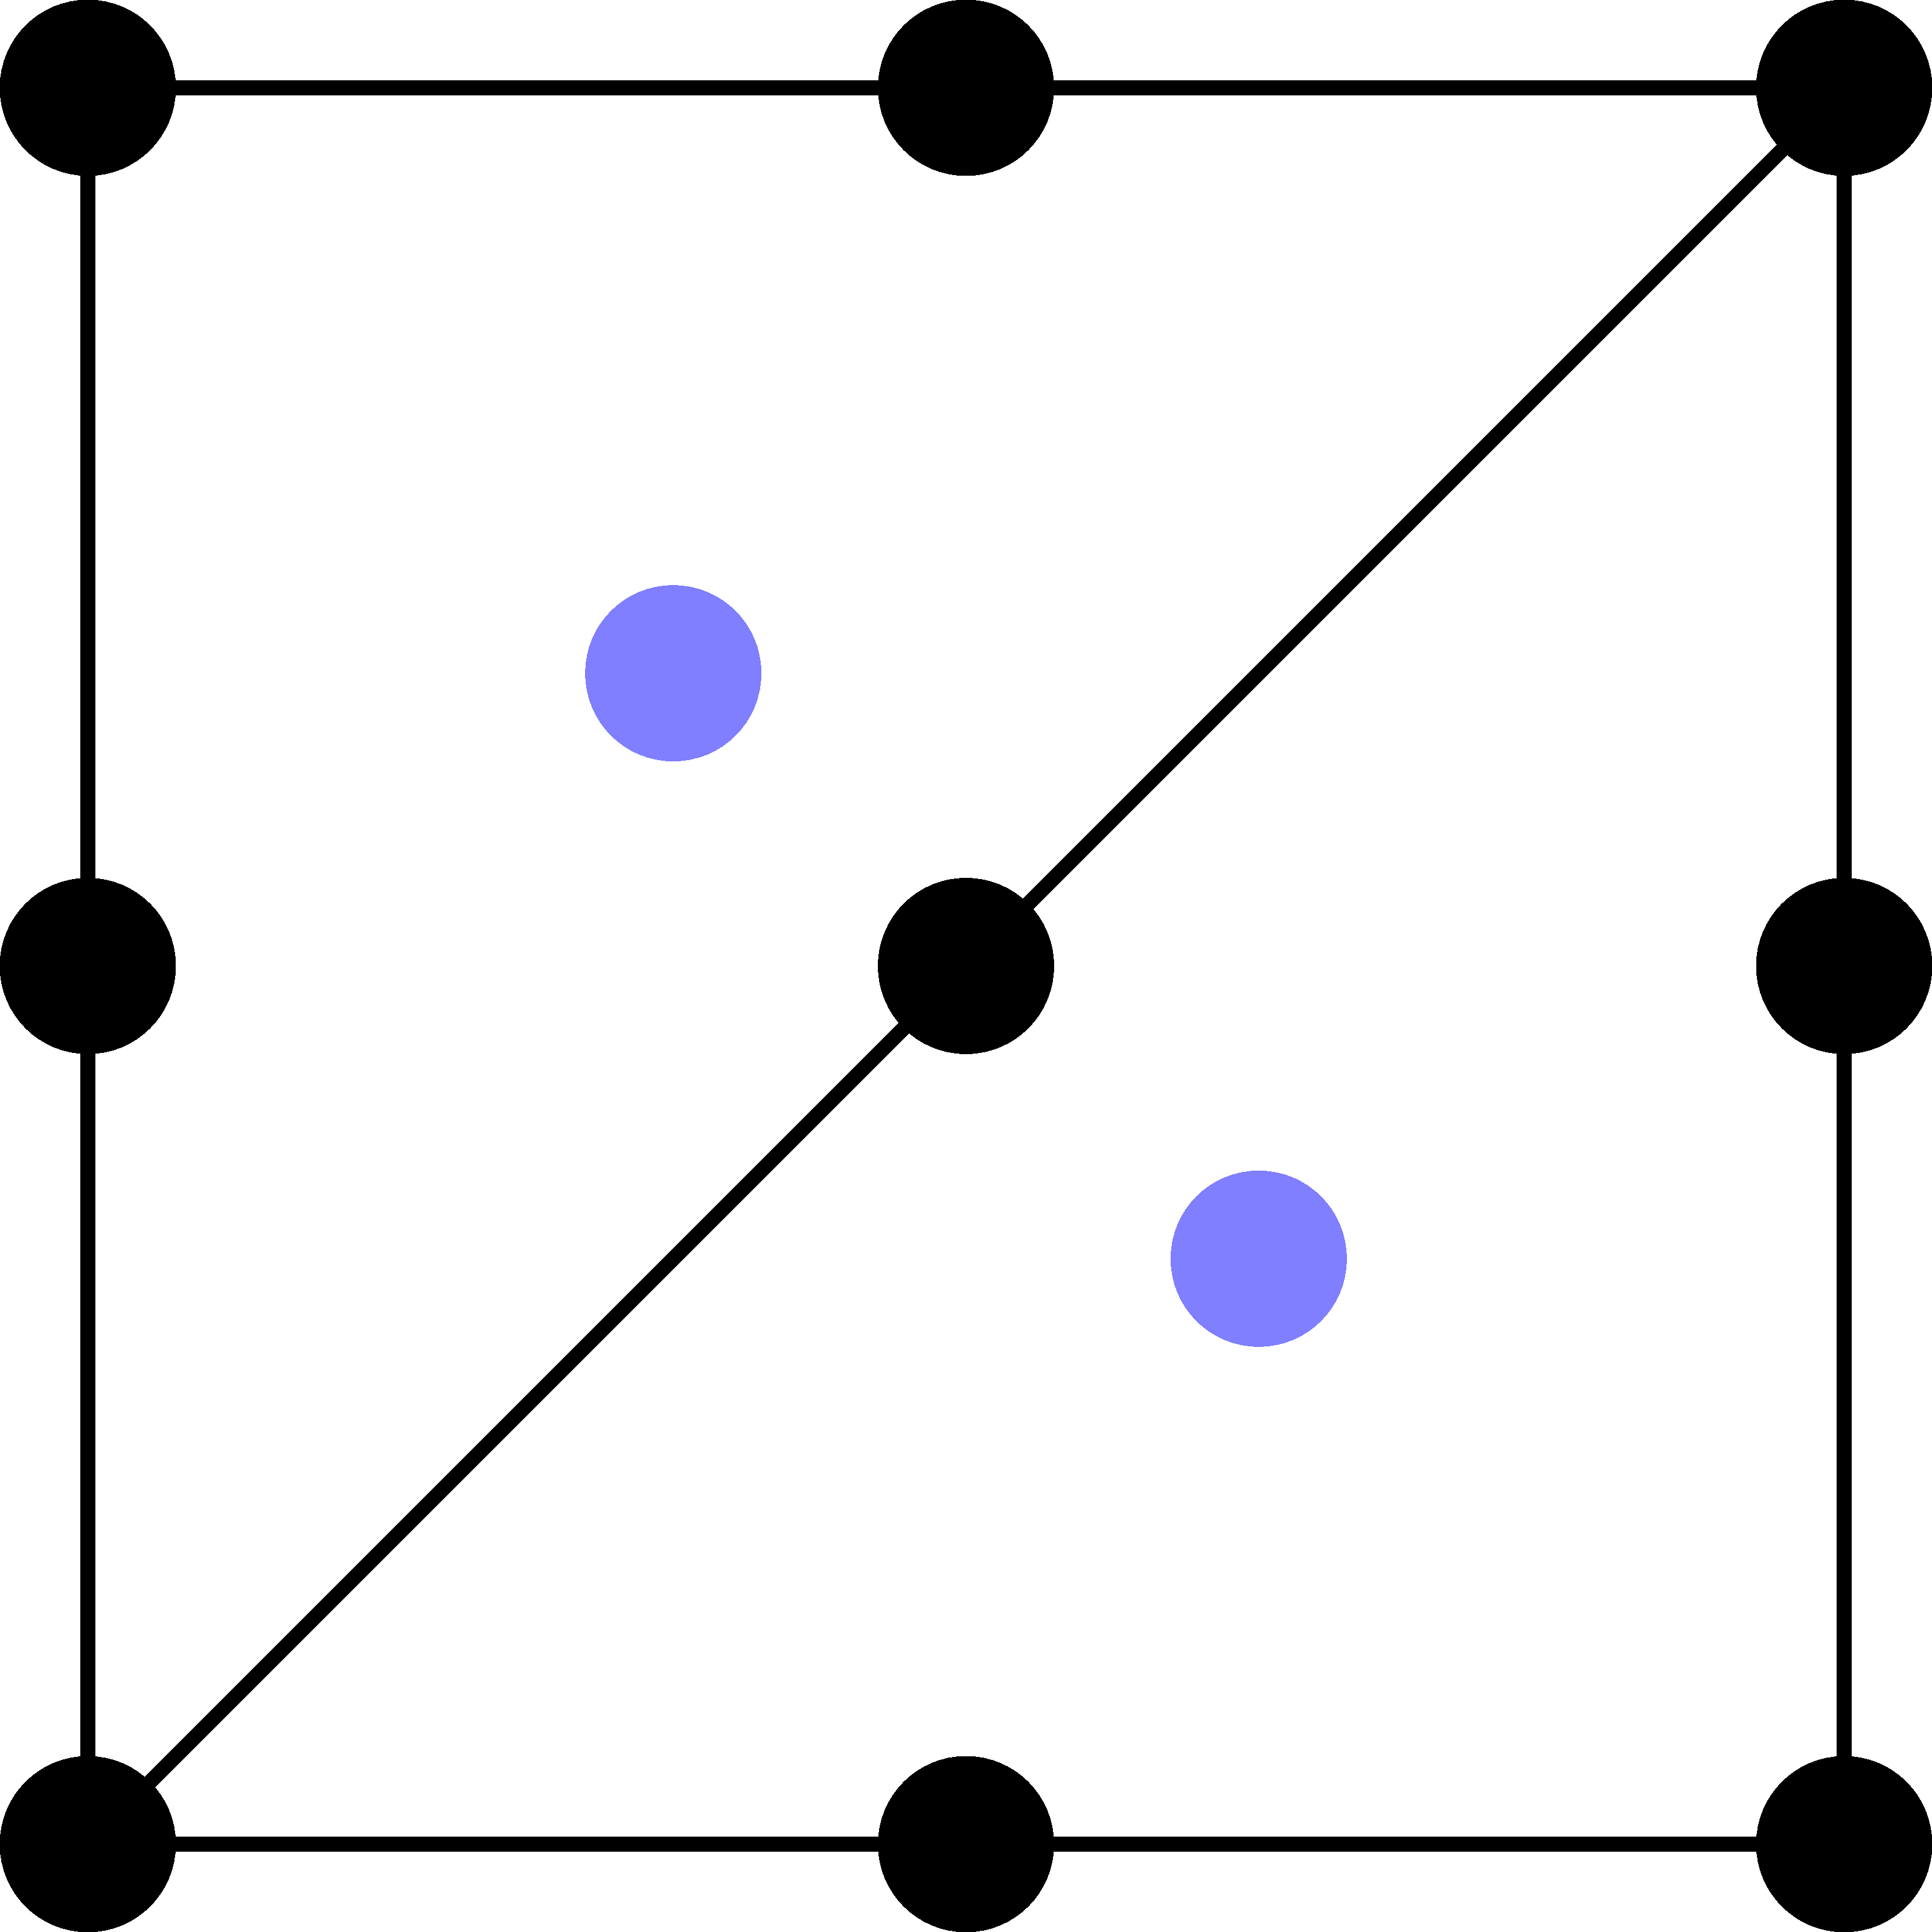
\includegraphics[width=0.9\textwidth]{figures/CrouzeixRaviart.png}
            \end{minipage}\\Crouzeix-Raviart element \cite{crouzeix1973}
        \end{tabular}
        &4&\checkmark & & \checkmark\\
        \hline
        \multicolumn{5}{c}{
                \begin{tabular}{c@{\hspace{24pt}}c}
                    \raisebox{-0.2\height}{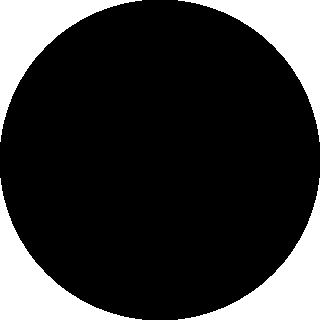
\includegraphics[width=10pt]{figures/legend_u.png}} :位移节点 &
                    \raisebox{-0.2\height}{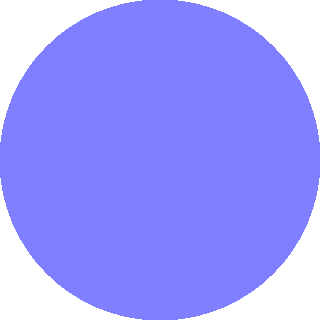
\includegraphics[width=10pt]{figures/legend_p.png}} :压力节点 
                \end{tabular}}\\
        \hline
    \end{tabular}
\end{table}

值得注意的是,从上述T3P1单元与Q4P1单元例子可以观察到,即使将两个单元中的压力节点数设置为最小值1,其仍然无法满足LBB稳定性条件。这一现象主要源于传统有限元离散方案中节点布置方式的固有局限性:在传统有限元混合离散方案中,压力节点必须依附于单元进行布置,且每个单元至少需要布置一个压力节点,这种限制导致节点数量无法根据位移节点与压力节点的最优比例需求进行灵活调整。因此,在传统有限元混合离散方案框架下,无论是三角形3位移节点单元还是四边形4位移节点单元,均不能满足LBB稳定性条件。

\section{小结}
本章对LBB稳定性条件进行了深入研究,通过结合特征值问题与体积约束比,推导出新的LBB稳定系数估算式,并确定了满足LBB稳定系数的最优体积约束比范围。首先,引入正交投影算子,推导出考虑刚度矩阵的最小非零特征值的LBB稳定系数估算式。随后,通过引入多项式空间,进一步推导出同时考虑特征值问题和体积约束自由度数量的LBB稳定系数估算式。在此基础上确定了满足LBB稳定性条件的最优体积约束比取值范围。并且,讨论了多项式空间中位移自由度和压力自由度的关系,并通过举例阐明了最优约束比下压力自由度数量的确定方法。通过规律总结了不同多项式空间阶数下的约束自由度数量,并建立了位移自由度与压力自由度数量之间的关系式,并举例说明了如何根据新方法确定混合离散单元是否满足LBB稳定性条件。为验证所提方法的有效性,采用系数估计法对多个经典单元进行了LBB稳定性条件验证,并将结果与数值验证结果、解析证明结果进行对比,充分证实了本文所提方法的正确性和可靠性。本章所提方法为验证LBB稳定性条件提供了更为简便直观的方法支持,对免体积自锁问题具有重要的意义。